\documentclass[fleqn,aspectratio=169,10pt]{beamer}
\usetheme{Madrid}
\usepackage[T1]{fontenc}
\begingroup
\catcode`_=\active
\gdef\literalunderscores #1{%
    \catcode`_=\active
    \def_{\_}%
    \scantokens{#1}%
}
\endgroup

\newcommand*{\cmd}[1]{\pmb{\mathrm{\protect\literalunderscores{#1}}}}
\newcommand*{\tvar}[1]{\mathrm{\mathit{\textrm{\textquotesingle}#1}}}
\newcommand*{\singlequote}{\textrm{\textquotesingle}}
\newcommand*{\type}[1]{\mathrm{\mathit{#1}}}
\newcommand*{\const}[1]{\mathrm{\mathsf{\protect\literalunderscores{#1}}}}
\newcommand*{\specon}[1]{\literalunderscores{#1}}
\newcommand*{\var}[1]{\mathrm{\mathit{#1}}}
\newcommand*{\syntax}[1]{\mathrm{\mathsf{\underline{#1}}}}
\newcommand*{\literal}[1]{\mathrm{\texttt{#1}}}

\newlength\isawidth
\newcommand*{\isabelleinner}{%
    \let\isaoldnewline=\\%
    \renewcommand{\\}{\setlength\isawidth{\linewidth}\isaoldnewline}%
    \setlength\isawidth{\linewidth}%
    \relpenalty=700%
}
\newenvironment{isabelle}{\list{}{}\item[]\isabelleinner}{\endlist}
\newenvironment{isabelle*}{\begingroup\isabelleinner}{\endgroup}
\newcommand*{\isa}[1]{\parbox[t]{\isawidth}{%
        \raggedright%
        \renewcommand{\\}{\isaoldnewline}%
        \setlength\hangindent{1em}%
        \strut \!\begin{align*}\displaystyle #1\end{align*}%
}}
\newcommand{\isabelleinline}[1]{$#1$}

\newcommand{\more}{\hspace*{1em}\addtolength{\isawidth}{-1em}}
\newcommand{\bmore}{\leavevmode\rlap{\hspace{0.2em}$|$}\more}
\newcommand{\less}{\hspace*{-1em}\more}
\newcommand{\bless}{\hspace*{-1em}\bmore}

\let\phi=\varphi
\newcommand{\oftype}{\mathrel{::}}
\newcommand{\Fun}{\Rightarrow}
\newcommand*{\PartialFun}{\rightharpoonup}
\newcommand{\Interval}{\mathcal{I}}
\newcommand{\Implies}{\longrightarrow}
\newcommand{\Forall}{\forall}
\newcommand{\Exists}{\exists}
\newcommand{\Andd}{\wedge}
%% \newcommand{\Or}{\lor}
\newcommand{\Iff}{\longleftrightarrow}

\mathcode`\#="2023
\mathcode`@="2040
\mathcode`!="2021
\newcommand{\Nil}{[\,]}
\newcommand{\Image}{\mathbin{\specon{\grave{}}}}
\newcommand{\InvImage}{\mathbin{{\text -}\const{\grave{}}}}
\newcommand{\MapThe}[1]{\overline{#1}}
\newcommand{\Upt}{\mathrel{..\mathrm{<}}}
\newcommand{\GreaterThanAtMost}{\mathrel{\mathrm{<}..}}
\newcommand{\None}{\bot}
\newcommand*{\Some}[1]{\langle #1\rangle}
\newcommand*{\Union}{\cup}
\newcommand*{\Intersection}{\cap}
\newcommand*{\Emptyset}{\{\}}

\newcommand{\Imp}{\rightarrow}
\newcommand{\Prev}{\operatorname{\CIRCLE}}
\newcommand{\Next}{\operatorname{\Circle}}
\newcommand{\Since}{\mathbin{\mathsf{S}}}
\newcommand{\Until}{\mathbin{\mathsf{U}}}
\newcommand{\Always}{\operatorname{\square}}
\newcommand{\PAlways}{\operatorname{\blacksquare}}
\newcommand{\Eventually}{\operatorname{\lozenge}}
\newcommand{\Once}{\operatorname{\blacklozenge}}

\newcommand{\SRel}{\const{Eq}_{\const{S}}}
\newcommand{\SPred}{\const{Pred}_{\const{S}}}
\newcommand{\SExists}{\const{Exists}_{\const{S}}}
\newcommand{\SAnd}{\const{And}_{\const{S}}}
\newcommand{\SOr}{\const{Or}_{\const{S}}}
\newcommand{\SNext}{\const{Next}_{\const{S}}}
\newcommand{\SPrev}{\const{Prev}_{\const{S}}}
\newcommand{\SSince}{\const{Since}_{\const{S}}}
\newcommand{\SUntil}{\const{Until}_{\const{S}}}

\newcommand{\Exfrm}{\phi_{\mathit{ex}}}
\newcommand{\Exprefix}{\pi_{\mathit{ex}}}

\newcommand*{\Univ}{\mathfrak{U}}

\newcommand*{\BulkBenq}[2]{{#1} \gg {#2}}

\newcommand*{\assoc}{\curvearrowleft}
\newcommand*{\reassoc}{\curvearrowright}

\newcommand*{\IdOp}{\mathcal{I}}
\newcommand*{\TranspOp}{\mathcal{X}}
\newcommand*{\Scomp}[2]{{#1} \bullet {#2}}
\newcommand*{\Pcomp}[2]{{#1} \parallel {#2}}
\newcommand*{\Feedback}[1]{{#1} \uparrow}
\newcommand*{\EndOp}{\oslash}
\newcommand*{\SilentOp}{\odot}
\newcommand*{\SpinOp}{\otimes}
\newcommand*{\SourceOp}{\rotatebox[origin=c]{180}{!}}
\newcommand*{\SinkOp}{!}
\newcommand*{\MergeOp}{\mathcal{V}}
\newcommand*{\SplitOp}{\Lambda}
\newcommand*{\AeqOp}{\mathcal{Q}}
\newcommand*{\AcopyOp}{\mathcal{C}}
\newcommand*{\PreBuf}{\dashv}
\newcommand*{\PostBuf}{\vdash}

\newcommand*{\bisim}[2]{{#1} \sim {#2}}
\newcommand*{\wbisim}[2]{{#1} \approx {#2}}
\newcommand*{\TraceEquiv}[2]{{#1} \equiv_t {#2}}

\newcommand*\highlight[1]{\mbox{\setlength{\fboxsep}{0pt}\colorbox{gray!30}{\strut$#1$}}}

\newcommand*{\circled}[1]{\tikz[baseline=(char.base)]{
  \node[shape=circle,draw,inner sep=0] (char) {#1};}}
\newcommand*{\ogt}{\circled{>}}
\newcommand*{\olt}{\circled{<}}


\setbeamertemplate{navigation symbols}{}

\setbeamertemplate{footline}
{
  \leavevmode%
  \hbox{%
  \begin{beamercolorbox}[wd=.4\paperwidth,ht=2.25ex,dp=1ex,center]{author in head/foot}%
    \usebeamerfont{author in head/foot}\insertshortauthor
  \end{beamercolorbox}%
  \begin{beamercolorbox}[wd=.6\paperwidth,ht=2.25ex,dp=1ex,center]{title in head/foot}%
    \usebeamerfont{title in head/foot}\insertshorttitle\hspace*{3em}
    \insertframenumber{} / \inserttotalframenumber\hspace*{1ex}
  \end{beamercolorbox}}%
  \vskip0pt%
}

\usepackage{wasysym}
\usepackage{fancybox,graphicx,hyperref,url}
\usepackage{tikz}
\usetikzlibrary{shapes,arrows}
\usetikzlibrary{positioning}
\usepackage{booktabs}
\usepackage{enumitem}
\usepackage{tikz}
\usetikzlibrary{decorations.markings,decorations.text,arrows.meta,arrows, shapes.geometric, arrows.meta, chains, decorations.markings, positioning, shadows }

\usepackage{listings}
\usepackage{pdfpages}
\usepackage{lstautogobble}

\usepackage[listings,skins,breakable,xparse,most,raster]{tcolorbox}
\tcbuselibrary{theorems}
\tcbset{highlight math/.append style={boxrule=0pt,
                                      frame hidden,
                                      colback=yellow!40!white,
                                      sharp corners}}

\usepackage{xpatch}

\usepackage{realboxes}
\usetikzlibrary{fit}
\usetikzlibrary{shadings}
\usetikzlibrary{shapes.arrows,shadows.blur}

\tikzset{
  operator/.style = {
  circle, draw, minimum size=1.3cm,
  % align = center
  },
  bigoperator/.style = {
  circle, draw, minimum size=1.8cm,
  % align = center
  },
  pics/transpA/.style = {
    code = {
      \node[bigoperator, label={[label distance=-1.2mm]90:\isabelleinline{\TranspOp}}] (op) {};
      \draw (op.70) ++ (0,-0.1mm) arc(-12:190:3.2mm);
      \draw[] (op.130) node [style = {circle, draw, fill, minimum size=2mm, inner sep=1pt}] (-il1) {};
      \draw[] (op.350) node [style = {circle, draw, fill, minimum size=2mm, inner sep=1pt}] (-ol1) {} ;
      \draw[] (op.150) node [style = {circle, draw, fill, minimum size=2mm, inner sep=1pt}] (-il2) {};
      \draw[] (op.330) node [style = {circle, draw, fill, minimum size=2mm, inner sep=1pt}] (-ol2) {} ;
      \draw[] (op.170) node [style = {circle, draw, fill, minimum size=2mm, inner sep=1pt}] (-il3) {};
      \draw[] (op.310) node [style = {circle, draw, fill, minimum size=2mm, inner sep=1pt}] (-ol3) {} ;

      \draw[] (op.230) node [style = {circle, draw, fill, minimum size=2mm, inner sep=1pt}] (-ir1) {};
      \draw[] (op.50) node [style = {circle, draw, fill, minimum size=2mm, inner sep=1pt}] (-or1) {} ;
      \draw [-] (-il1) to (-ol1);
      \draw [-, postaction={decoration={
            text effects along path,
            text={{}{\(l_1\)}},
            text align=left,
            text effects/.cd,
            text along path,
            characters={fill=white, yshift=-0.6ex, xshift=+0.5ex},
          }, decorate}] (-il2) to (-ol2);
      \draw [-,postaction={decoration={
            text effects along path,
            text={{}{\(r_1\)}},
            text align=left,
            text effects/.cd,
            text along path,
            characters={fill=white, yshift=-0.6ex, xshift=+0.5ex},
          }, decorate}] (-ir1) to (-or1);
      \draw [-] (-il3) to (-ol3);
    }
  },
  pics/transpB/.style = {
    code = {
      \node[bigoperator, label={[label distance=-1.2mm]90:\isabelleinline{\TranspOp}}] (op) {};
      \draw (op.70) ++ (0,-0.1mm) arc(-12:190:3.2mm);
      \draw[] (op.190) node [style = {circle, draw, fill, minimum size=2mm, inner sep=1pt}] (-ir1) {};
      \draw[] (op.50) node [style = {circle, draw, fill, minimum size=2mm, inner sep=1pt}] (-or1) {} ;
      \draw[] (op.210) node [style = {circle, draw, fill, minimum size=2mm, inner sep=1pt}] (-ir2) {};
      \draw[] (op.30) node [style = {circle, draw, fill, minimum size=2mm, inner sep=1pt}] (-or2) {} ;
      \draw[] (op.230) node [style = {circle, draw, fill, minimum size=2mm, inner sep=1pt}] (-ir3) {};
      \draw[] (op.10) node [style = {circle, draw, fill, minimum size=2mm, inner sep=1pt}] (-or3) {} ;

      \draw[] (op.130) node [style = {circle, draw, fill, minimum size=2mm, inner sep=1pt}] (-il1) {};
      \draw[] (op.310) node [style = {circle, draw, fill, minimum size=2mm, inner sep=1pt}] (-ol1) {} ;
      \draw [-,postaction={decoration={
            text effects along path,
            text={{}{\(r_3\)}},
            text align=left,
            text effects/.cd,
            text along path,
            characters={fill=white, yshift=-0.6ex, xshift=+0.5ex},
          }, decorate}] (-il1) to (-ol1);
      \draw [-] (-ir1) to (-or1);
      \draw [-, postaction={decoration={
            text effects along path,
            text={{}{\(l_3\)}},
            text align=left,
            text effects/.cd,
            text along path,
            characters={fill=white, yshift=-0.6ex, xshift=+0.5ex},
          }, decorate}] (-ir2) to (-or2);
      \draw [-] (-ir3) to (-or3);
    }
  },
  pics/idA/.style = {
    code = {
      \node[bigoperator, label={[label distance=-1.2mm]90:\isabelleinline{\IdOp}}] (op) {};
      \draw (op.70) ++ (0,-0.1mm) arc(-12:190:3.2mm);
      \draw[] (op.130) node [style = {circle, draw, fill, minimum size=2mm, inner sep=1pt}] (-il1) {};
      \draw[] (op.50) node [style = {circle, draw, fill, minimum size=2mm, inner sep=1pt}] (-ol1) {} ;
      \draw[] (op.150) node [style = {circle, draw, fill, minimum size=2mm, inner sep=1pt}] (-il2) {};
      \draw[] (op.30) node [style = {circle, draw, fill, minimum size=2mm, inner sep=1pt}] (-ol2) {} ;
      \draw[] (op.170) node [style = {circle, draw, fill, minimum size=2mm, inner sep=1pt}] (-il3) {};
      \draw[] (op.10) node [style = {circle, draw, fill, minimum size=2mm, inner sep=1pt}] (-ol3) {} ;

      \draw[] (op.230) node [style = {circle, draw, fill, minimum size=2mm, inner sep=1pt}] (-ir1) {};
      \draw[] (op.310) node [style = {circle, draw, fill, minimum size=2mm, inner sep=1pt}] (-or1) {} ;
      \draw [-, postaction={decoration={
            text effects along path,
            text={{}{\(l\)}},
            text align=center,
            text effects/.cd,
            text along path,
            characters={fill=white, yshift=-0.6ex},
          }, decorate}] (-il2) to (-ol2);
      \draw [-] (-il1) to (-ol1);
      \draw [-,postaction={decoration={
            text effects along path,
            text={{}{\(r\)}},
            text align=center,
            text effects/.cd,
            text along path,
            characters={fill=white, yshift=-0.4ex},
          }, decorate}] (-ir1) to (-or1);
      \draw [-] (-il3) to (-ol3);
    }
  },
  pics/aeqA/.style = {
    code = {
      \node[operator, label={[label distance=-1.3mm]90:\isabelleinline{\AeqOp_0}}] (op) {};
      \draw (op.60) ++ (0,-0.1mm) arc(-12:190:3.4mm);
      \draw[] (op.150) node [style = {circle, draw, fill, minimum size=2mm, inner sep=1pt}] (-il) {};

      \draw[] (op.210) node [style = {circle, draw, fill, minimum size=2mm, inner sep=1pt}] (-ir) {};

      \draw[] (op.0) node [style = {circle, draw, fill, minimum size=2mm, inner sep=1pt}] (-o) {} ;

      \draw [-, postaction={decoration={
            text effects along path,
            text={{}{\(x\)}},
            text align=center,
            text effects/.cd,
            text along path,
            characters={fill=white, yshift=-0.6ex, xshift=-0.5ex},
          }, decorate}] (-il) to (-o);
      \draw [-,postaction={decoration={
            text effects along path,
            text={{}{\(y\)}},
            text align=center,
            text effects/.cd,
            text along path,
            characters={fill=white, yshift=-0.4ex, xshift=-0.5ex},
          }, decorate}] (-ir) to (-o);
    }
  },
  pics/acopyA/.style = {
    code = {
      \node[operator, label={[label distance=-1.3mm]90:\isabelleinline{\AcopyOp_0}}] (op) {};
      \draw (op.60) ++ (0,-0.1mm) arc(-12:190:3.4mm);
      \draw[] (op.180) node [style = {circle, draw, fill, minimum size=2mm, inner sep=1pt}] (-i) {};

      \draw[] (op.30) node [style = {circle, draw, fill, minimum size=2mm, inner sep=1pt}] (-ol) {} ;
      \draw[] (op.330) node [style = {circle, draw, fill, minimum size=2mm, inner sep=1pt}] (-or) {} ;

      \draw [-, postaction={decoration={
            text effects along path,
            text={{}{\(v\)}},
            text align=center,
            text effects/.cd,
            text along path,
            characters={fill=white, yshift=-0.6ex, xshift=+0.5ex},
          }, decorate}] (-i) to (-ol);
      \draw [-,postaction={decoration={
            text effects along path,
            text={{}{\(w\)}},
            text align=center,
            text effects/.cd,
            text along path,
            characters={fill=white, yshift=-0.4ex, xshift=+0.5ex},
          }, decorate}] (-i) to (-or);
    }
  },
  pics/acopyB/.style = {
    code = {
      \node[operator, label={[label distance=-1.3mm]90:\isabelleinline{\AcopyOp_1}}] (op) {};
      \draw (op.60) ++ (0,-0.1mm) arc(-12:190:3.4mm);
      \draw[] (op.180) node [style = {circle, draw, fill, minimum size=2mm, inner sep=1pt}] (-i) {};

      \draw[] (op.30) node [style = {circle, draw, fill, minimum size=2mm, inner sep=1pt}] (-ol) {} ;
      \draw[] (op.330) node [style = {circle, draw, fill, minimum size=2mm, inner sep=1pt}] (-or) {} ;

      \draw [-, postaction={decoration={
            text effects along path,
            text={{}{\(a_1\)}},
            text align=center,
            text effects/.cd,
            text along path,
            characters={fill=white, yshift=-0.6ex, xshift=+1.9ex},
          }, decorate}] (-i) to (-ol);
      \draw [-,postaction={decoration={
            text effects along path,
            text={{}{\(b_1\)}},
            text align=center,
            text effects/.cd,
            text along path,
            characters={fill=white, yshift=-0.4ex, xshift=+1.9ex},
          }, decorate}] (-i) to (-or);
    }
  },
  pics/acopyC/.style = {
    code = {
      \node[operator, label={[label distance=-1.3mm]90:\isabelleinline{\AcopyOp_2}}] (op) {};
      \draw (op.60) ++ (0,-0.1mm) arc(-12:190:3.4mm);
      \draw[] (op.180) node [style = {circle, draw, fill, minimum size=2mm, inner sep=1pt}] (-i) {};

      \draw[] (op.30) node [style = {circle, draw, fill, minimum size=2mm, inner sep=1pt}] (-ol) {} ;
      \draw[] (op.330) node [style = {circle, draw, fill, minimum size=2mm, inner sep=1pt}] (-or) {} ;

      \draw [-, postaction={decoration={
            text effects along path,
            text={{}{\(c_1\)}},
            text align=center,
            text effects/.cd,
            text along path,
            characters={fill=white, yshift=-0.6ex, xshift=+1.9ex},
          }, decorate}] (-i) to (-ol);
      \draw [-,postaction={decoration={
            text effects along path,
            text={{}{\(d_1\)}},
            text align=center,
            text effects/.cd,
            text along path,
            characters={fill=white, yshift=-0.4ex, xshift=+1.9ex},
          }, decorate}] (-i) to (-or);
    }
  },
  pics/transpC/.style = {
    code = {
      \node[operator, label={[label distance=-1.3mm]90:\isabelleinline{\TranspOp_0}}] (op) {};
      \draw (op.60) ++ (0,-0.1mm) arc(-12:190:3.4mm);
      \draw[] (op.140) node [style = {circle, draw, fill, minimum size=2mm, inner sep=1pt}] (-il) {};
      \draw[] (op.320) node [style = {circle, draw, fill, minimum size=2mm, inner sep=1pt}] (-or) {} ;

      \draw[] (op.220) node [style = {circle, draw, fill, minimum size=2mm, inner sep=1pt}] (-ir) {};
      \draw[] (op.40) node [style = {circle, draw, fill, minimum size=2mm, inner sep=1pt}] (-ol) {} ;
      \draw [-,postaction={decoration={
            text effects along path,
            text={{}{\(c_3\)}},
            text align=left,
            text effects/.cd,
            text along path,
            characters={fill=white, yshift=-0.6ex, xshift=+0.5ex},
          }, decorate}] (-ir) to (-ol);
      \draw [-, postaction={decoration={
            text effects along path,
            text={{}{\(b_3\)}},
            text align=left,
            text effects/.cd,
            text along path,
            characters={fill=white, yshift=-0.6ex, xshift=+0.5ex},
          }, decorate}] (-il) to (-or);
    }
  },
  pics/idB/.style = {
    code = {
      \node[operator, label={[label distance=-1.3mm]90:\isabelleinline{\IdOp_0}}] (op) {};
      \draw (op.60) ++ (0,-0.1mm) arc(-12:190:3.4mm);
      \draw[] (op.180) node [style = {circle, draw, fill, minimum size=2mm, inner sep=1pt}] (-i) {};

      \draw[] (op.0) node [style = {circle, draw, fill, minimum size=2mm, inner sep=1pt}] (-o) {} ;

      \draw [-,postaction={decoration={
            text effects along path,
            text={{}{\(a_3\)}},
            text align=center,
            text effects/.cd,
            text along path,
            characters={fill=white, yshift=-0.4ex},
          }, decorate}] (-i) to (-o);
    }
  },
  pics/idC/.style = {
    code = {
      \node[operator, label={[label distance=-1.3mm]90:\isabelleinline{\IdOp_1}}] (op) {};
      \draw (op.60) ++ (0,-0.1mm) arc(-12:190:3.4mm);
      \draw[] (op.180) node [style = {circle, draw, fill, minimum size=2mm, inner sep=1pt}] (-i) {};

      \draw[] (op.0) node [style = {circle, draw, fill, minimum size=2mm, inner sep=1pt}] (-o) {} ;

      \draw [-,postaction={decoration={
            text effects along path,
            text={{}{\(d_3\)}},
            text align=center,
            text effects/.cd,
            text along path,
            characters={fill=white, yshift=-0.4ex},
          }, decorate}] (-i) to (-o);
    }
  },
  pics/idD/.style = {
    code = {
      \node[operator, label={[label distance=-1.3mm]90:\isabelleinline{\IdOp_3}}] (op) {};
      \draw (op.60) ++ (0,-0.1mm) arc(-12:190:3.4mm);
      \draw[] (op.180) node [style = {circle, draw, fill, minimum size=2mm, inner sep=1pt}] (-i) {};

      \draw[] (op.0) node [style = {circle, draw, fill, minimum size=2mm, inner sep=1pt}] (-o) {} ;

      \draw [-,postaction={decoration={
            text effects along path,
            text={{}{\(bd_2\)}},
            text align=center,
            text effects/.cd,
            text along path,
            characters={fill=white, yshift=-0.4ex},
          }, decorate}] (-i) to (-o);
    }
  },
  pics/idE/.style = {
    code = {
      \node[operator, label={[label distance=-1.3mm]90:\isabelleinline{\IdOp_2}}] (op) {};
      \draw (op.60) ++ (0,-0.1mm) arc(-12:190:3.4mm);
      \draw[] (op.180) node [style = {circle, draw, fill, minimum size=2mm, inner sep=1pt}] (-i) {};

      \draw[] (op.0) node [style = {circle, draw, fill, minimum size=2mm, inner sep=1pt}] (-o) {} ;

      \draw [-,postaction={decoration={
            text effects along path,
            text={{}{\(ac_2\)}},
            text align=center,
            text effects/.cd,
            text along path,
            characters={fill=white, yshift=-0.4ex},
          }, decorate}] (-i) to (-o);
    }
  },
  pics/aeqB/.style = {
    code = {
      \node[operator, label={[label distance=-1.3mm]90:\isabelleinline{\AeqOp_1}}] (op) {};
      \draw (op.60) ++ (0,-0.1mm) arc(-12:190:3.4mm);
      \draw[] (op.150) node [style = {circle, draw, fill, minimum size=2mm, inner sep=1pt}] (-il) {};

      \draw[] (op.210) node [style = {circle, draw, fill, minimum size=2mm, inner sep=1pt}] (-ir) {};

      \draw[] (op.0) node [style = {circle, draw, fill, minimum size=2mm, inner sep=1pt}] (-o) {} ;

      \draw [-, postaction={decoration={
            text effects along path,
            text={{}{\(a_5\)}},
            text align=center,
            text effects/.cd,
            text along path,
            characters={fill=white, yshift=-0.6ex, xshift=-1.9ex},
          }, decorate}] (-il) to (-o);
      \draw [-,postaction={decoration={
            text effects along path,
            text={{}{\(c_5\)}},
            text align=center,
            text effects/.cd,
            text along path,
            characters={fill=white, yshift=-0.4ex, xshift=-1.9ex},
          }, decorate}] (-ir) to (-o);
    }
  },
  pics/aeqC/.style = {
    code = {
      \node[operator, label={[label distance=-1.3mm]90:\isabelleinline{\AeqOp_2}}] (op) {};
      \draw (op.60) ++ (0,-0.1mm) arc(-12:190:3.4mm);
      \draw[] (op.150) node [style = {circle, draw, fill, minimum size=2mm, inner sep=1pt}] (-il) {};

      \draw[] (op.210) node [style = {circle, draw, fill, minimum size=2mm, inner sep=1pt}] (-ir) {};

      \draw[] (op.0) node [style = {circle, draw, fill, minimum size=2mm, inner sep=1pt}] (-o) {} ;

      \draw [-,postaction={decoration={
            text effects along path,
            text={{}{\(d_5\)}},
            text align=center,
            text effects/.cd,
            text along path,
            characters={fill=white, yshift=-0.4ex, xshift=-1.9ex},
          }, decorate}] (-ir) to (-o);
      \draw [-, postaction={decoration={
            text effects along path,
            text={{}{\(b_5\)}},
            text align=center,
            text effects/.cd,
            text along path,
            characters={fill=white, yshift=-0.6ex, xshift=-1.9ex},
          }, decorate}] (-il) to (-o);
    }
  },
  pics/aeqop21/.style = {
    code = {
      \node[operator, label={[label distance=-1.3mm]90:\isabelleinline{\AeqOp}}] (op) {};
      \draw[] (op.135) node [style = {circle, draw, fill, minimum size=2mm,
      inner sep=1pt}] (-i1) {} -- node [style = {circle, draw, fill, minimum
      size=2mm, inner sep=1pt}] (-o) {} (op.0);
      \draw[] (op.225) node [style = {circle, draw, fill, minimum size=2mm,
      inner sep=1pt}] (-i2) {} -- (op.0);
    }
  },
  pics/acopyop12/.style = {
    code = {
      \node[operator, label={[label distance=-1.3mm]90:\isabelleinline{\AcopyOp}}] (op) {};
      \draw (op.60) ++ (0,-0.1mm) arc(-12:190:3.2mm);
      \draw[] (op.180) node [style = {circle, draw, fill, minimum size=2mm,
      inner sep=1pt}] (-i) {} -- node [style = {circle, draw, fill, minimum
      size=2mm, inner sep=1pt}] (-o1) {} (op.45);
      \draw[] (op.180) -- node [style = {circle, draw, fill, minimum size=2mm,
      inner sep=1pt}] (-o2) {} (op.315);
    }
  },
  pics/mergeop21/.style = {
    code = {
      \node[operator, label={[label distance=-1.3mm]90:\isabelleinline{\MergeOp}}] (op) {};
      \draw (op.60) ++ (0,-0.1mm) arc(-12:190:3.2mm);
      \draw[] (op.135) node [style = {circle, draw, fill, minimum size=2mm,
      inner sep=1pt}] (-i1) {} -- node [style = {circle, draw, fill, minimum
      size=2mm, inner sep=1pt}] (-o) {} (op.0);
      \draw[] (op.225) node [style = {circle, draw, fill, minimum size=2mm,
      inner sep=1pt}] (-i2) {} -- (op.0);
    }
  },
  pics/splitop12/.style = {
    code = {
      \node[operator, label={[label distance=-1.3mm]90:\isabelleinline{\SplitOp}}] (op) {};
      \draw (op.60) ++ (0,-0.1mm) arc(-12:190:3.2mm);
      \draw[] (op.180) node [style = {circle, draw, fill, minimum size=2mm,
      inner sep=1pt}] (-i) {} -- node [style = {circle, draw, fill, minimum
      size=2mm, inner sep=1pt}] (-o1) {} (op.45);
      \draw[] (op.180) -- node [style = {circle, draw, fill, minimum size=2mm,
      inner sep=1pt}] (-o2) {} (op.315);
    }
  },
}

\pgfdeclarefunctionalshading{Hermite-Gaussian modes}{\pgfpoint{-25bp}{-25bp}}{\pgfpoint{25bp}{25bp}}{}{
    10 atan sin 1000 mul cos 1 add
    exch
    10 atan sin 1000 mul cos 1 add
    mul 4 div
    dup dup
}

\makeatletter
\xpretocmd\lstinline{\Colorbox{yellow!10!white}\bgroup\appto\lst@DeInit{\egroup}}{}{}
\makeatother

\definecolor{my_red}{RGB}{128, 0, 0}

\lstset{captionpos=b}
\lstset{numberbychapter=false}
\lstset{autogobble}
% \lstset{breaklines=true}

\usepackage{tikz}
\usepackage{subcaption}
\usetikzlibrary{calc, chains, decorations.pathmorphing}
\usetikzlibrary{shapes,arrows,backgrounds}
\usetikzlibrary{positioning,fit,shapes.geometric,shapes}

\setbeamercovered{transparent}

\setlistdepth{9}
\setlist[itemize,1]{label=$\bullet$}
\setlist[itemize,2]{label=$\bullet$}
\setlist[itemize,3]{label=$\bullet$}
\setlist[itemize,4]{label=$\bullet$}
\setlist[itemize,5]{label=$\bullet$}
\setlist[itemize,6]{label=$\bullet$}
\setlist[itemize,7]{label=$\bullet$}
\setlist[itemize,8]{label=$\bullet$}
\setlist[itemize,9]{label=$\bullet$}
\renewlist{itemize}{itemize}{9}

\setlist[enumerate,1]{label=$\arabic*.$}
\setlist[enumerate,2]{label=$\alph*.$}
\setlist[enumerate,3]{label=$\roman*.$}
\setlist[enumerate,4]{label=$\arabic*.$}
\setlist[enumerate,5]{label=$\alpha*$}
\setlist[enumerate,6]{label=$\roman*.$}
\setlist[enumerate,7]{label=$\arabic*.$}
\setlist[enumerate,8]{label=$\alph*.$}
\setlist[enumerate,9]{label=$\roman*.$}
\renewlist{enumerate}{enumerate}{9}

\AtBeginSection[]{
  \begin{frame}[noframenumbering]
    \vfill
    \centering
    \begin{beamercolorbox}[sep=8pt,center,shadow=true,rounded=true]{title}
      \usebeamerfont{title}\insertsectionhead\par%
    \end{beamercolorbox}
    \vfill
  \end{frame}
}

\title[Nondeterministic Asynchronous Dataflow in Isabelle/HOL]{Nondeterministic Asynchronous Dataflow in Isabelle/HOL}

\author[\underline{Rafael}, Laouen and, Dmitriy]{
  \underline{Rafael Castro G. Silva}, Laouen Fernet and,  Dmitriy Traytel\\\medskip
  }
% {\small \url{rasi@di.ku.dk}}

\date{14/05/2025}

% change title (done)
% (co)datatypes -> codatatypes (done)
% while_option from HOL library (done)
% coindtive principle -> coinduction principle (done)
% remove next step slide, andd as a bullet (done)
% explain slice in more detail (done)
% mention selectors in llist slide, drop lmap, drop lset (done)
% move count operator example to slide that introduce op type (done)
% modeling lazy list processors which do not care about time (done)
% reduce Corecursion is like recursion line (done)
% why partial order? mention timely dataflow (done)
% explain what incremental, and set expectation for example (done)
% move arrows (done)
% Change push to out, done to out (done)
% put star footnote on op type saying it is simplified compare to the paper, also in the composition lemma (done)
% write the lapp lemma about lfinite (done)
% show coinduction principle for llist (done)
% add link llist afp (done)
% on produce slide, metion lshift as friend (point to freinds with benefits paper) (done)
% justify the compositional reasoning with lines of code for each building block (done)
% slide about tecnicques used, coinduction principles, friends, reasoning up to friends, generalization using skip_op, combining coinduction and induction, coinduction up to congruence for coinductive predicates, say our paper is more detailed in these topics
%
% add definition of batch_op, and all 4 properties

\institute[UCPH]{
  Department of Computer Science \\
  University of Copenhagen}

\begin{document}
\setbeamercovered{invisible}
% \setbeamercovered{dynamic}

\begin{frame}
  \titlepage
\end{frame}

\section{Motivation}

\begin{frame}[fragile]
  \frametitle{Motivation}
  \begin{block}{Context:}
  \begin{itemize}
    \item Stream Processing: programs that compute (possibly) unbounded sequences of data (streams)
    \item Frameworks: Google Cloud Dataflow, Apache Flink, and Timely Dataflow
          \begin{figure}
            \centering
            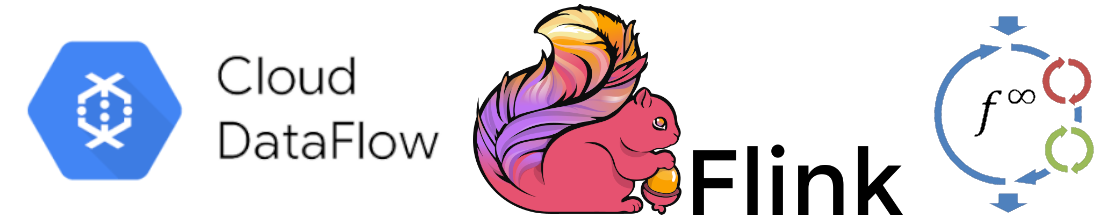
\includegraphics[scale=0.1]{all}
          \end{figure}
    % \item Why use frameworks?
    %       \begin{itemize}
    %         \item Highly Parallel
    %         \item Low latency (output as soon as possible)
    %         \item Incremental computing (re-uses previous computations)
    %       \end{itemize}
  \end{itemize}
  \pause
  \end{block}
  \begin{block}{Our long term goal:}
    Mechanically Verify Timely Dataflow algorithms
  \end{block}
\end{frame}

\section{A Good Foundation}

\begin{frame}[fragile]
  \frametitle{A Good Foundation}
  \begin{columns}
    \begin{column}{.35\textwidth}
      \begin{figure}
        \centering
        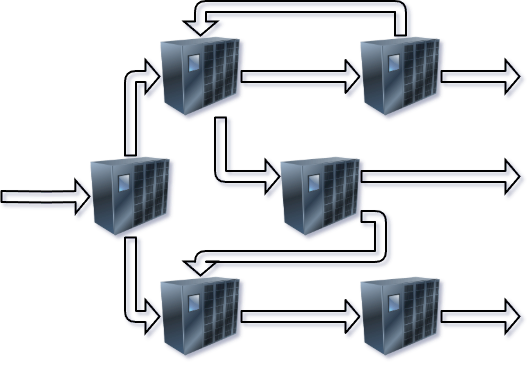
\includegraphics[width=1\textwidth]{network.png}
      \end{figure}
    \end{column}
    \begin{column}{.65\textwidth}
      \begin{itemize}
        \item Nondeterministic Asynchronous Dataflow
              \begin{itemize}
                \pause
                \item Dataflow: Directed graph of interconnected operators
                \pause
                \item Asynchronous:
                      \begin{itemize}
                        \item Operators execute independently:\\ processes without an orchestrator
                        \item Operators can freely communicate with the network (read/write); do silent computation steps
                        \item Networks are unbounded FIFO queues
                      \end{itemize}
                \pause
                \item Nondeterministic:
                      \begin{itemize}
                        \item Operators can make nondeterministic choices
                      \end{itemize}
              \end{itemize}
      \end{itemize}
    \end{column}
  \end{columns}
  \pause
  \begin{block}{Question}
    How do we know something is Nondeterministic Asynchronous Dataflow?
  \end{block}
\end{frame}

\begin{frame}[fragile]
  \frametitle{The Algebra for Nondeterministic Asynchronous Dataflow}
  \begin{columns}
    \begin{column}{.6\textwidth}
      \begin{itemize}
        \item Bergstra et al. presents an algebra for Nondeterministic Asynchronous Dataflow
        \item Primitives:\\
              sequential and parallel composition; feedback loop...
        \item 52 axioms
        \item A process calculus instance
      \end{itemize}
    \end{column}
    \begin{column}{.4\textwidth}
      \begin{figure}
        \centering
        \shadowbox{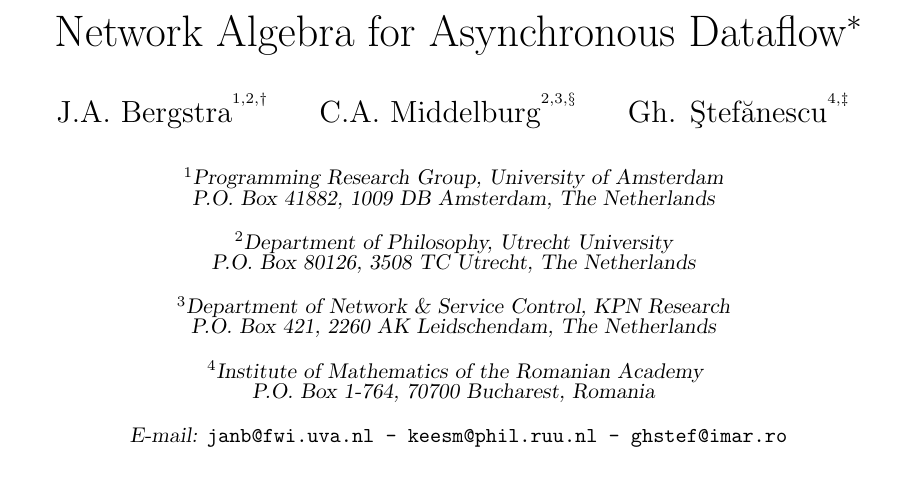
\includegraphics[width=0.9\textwidth]{Bergstra.png}}
      \end{figure}
    \end{column}
  \end{columns}
\end{frame}

\begin{frame}[fragile]
  \frametitle{Main Contributions}
  \begin{itemize}
    \item An Isabelle/HOL instance of Nondeterministic Asynchronous Dataflow
          \begin{itemize}
            \item Operators as a shallow embedding as codatatypes
            \item 51 axioms proved
          \end{itemize}
    % \item Executable via code extraction to Haskell
  \end{itemize}
\end{frame}

\section{Isabelle/HOL Preliminaries}

\begin{frame}[fragile]
  \frametitle{What is Isabelle/HOL?}
  \pause
  \begin{itemize}
    \item Isabelle: A generic proof assistant
          \begin{overlayarea}{\textwidth}{.3\textheight}
            \centering
            \begin{figure}
              \centering
              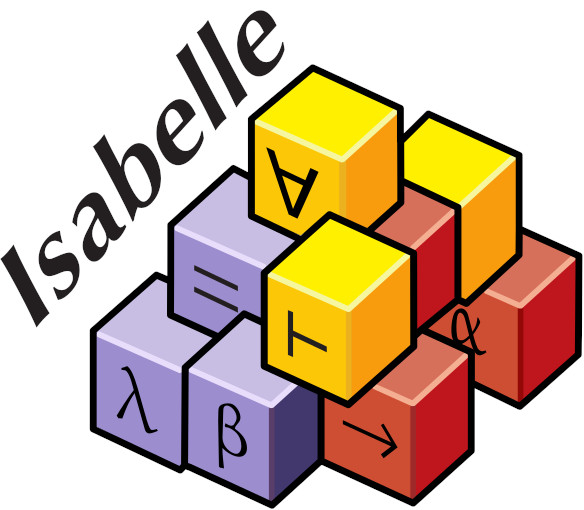
\includegraphics[scale=0.15]{isabelle}
            \end{figure}
          \end{overlayarea}
    \item Classical higher-order logic (HOL):\\ Simple Typed Lambda Calculus + axiom of choice + axiom of infinity + rank-1 polymorphism
          \pause
    \item Isabelle/HOL: Isabelle's flavor of HOL
  \end{itemize}
  \pause
    \begin{block}{Why Isabelle/HOL?}
      \begin{itemize}
        \item Codatatypes: (possibly) infinite data structures (e.g., lazy lists, streams)
        \item Corecursion: always eventually produces some codatatype constructor
        \item Coinductive predicates: infinite number of introduction rule applications
        \item Coinduction: reason about coinductive predicates
      \end{itemize}
  \end{block}

\end{frame}

\section{Operators as a Codatatype}

\begin{frame}[fragile]
  \frametitle{Operators}
  \vspace*{-2ex}
  \begin{tcolorbox}[enhanced,title=Operators in Isabelle/HOL,colback=yellow!30]
    \vspace*{-3ex}
    \hspace*{-5ex}
    \begin{align*}
      &   \cmd{codatatype}\ (\tvar{i}, \tvar{o}, \tvar{d})\ \type{op} =\\
      &   \more \const{Read}\ \tvar{i}\ (\tvar{d} \Fun (\tvar{i}, \tvar{o}, \tvar{d})\ \type{op})\ |\ \const{Write}\ ((\tvar{i}, \tvar{o}, \tvar{d})\ \type{op})\ \tvar{o}\ \tvar{d}\\
      &   \more \const{Silent}\ (\tvar{i}, \tvar{o}, \tvar{d})\ \type{op}\ |\ \const{Choice}\ ((\tvar{i}, \tvar{o}, \tvar{d})\ \type{op})\ \type{cset}
    \end{align*}
  \end{tcolorbox}

  \begin{columns}
    \begin{column}{.3\textwidth}
      \pause
      \begin{itemize}
        \item Type parameters: \\
              inputs/output ports; data
        \item Operator's actions
        % \item inputs/outputs: \\
        %       Sets of used ports
        \item Possibly infinite trees
      \end{itemize}
    \end{column}
    \begin{column}{.22\textwidth}
      \pause
      \begin{tcolorbox}[enhanced,title=Uncommunicative operators,colback=yellow!30]
        \vspace*{-5ex}
        \hspace*{-8ex}
        \begin{tabular}{l l l}
          \hspace*{-4ex}
          \isa{
          & \more \EndOp = \const{Choice}\ \{\}_c
            }&
          \vspace*{-5ex}
          \\
          \hspace*{-4ex}
          \isa{
          & \more \SilentOp = \const{Silent}\ \SilentOp
            }&
          \vspace*{-5ex}
          \\
          \hspace*{-4ex}
          \isa{
          & \more \SpinOp = \const{Choice}\ \{\SpinOp\}_c
            }
        \end{tabular}
        \vspace*{-1ex}
      \end{tcolorbox}
    \end{column}
    \begin{column}{.48\textwidth}
      \pause
      \begin{tcolorbox}[enhanced,title=More examples,colback=yellow!30]
        \vspace*{-5ex}
        \hspace*{-8ex}
        \begin{tabular}{l l l}
          \hspace*{-2ex}
          \isa{
          \const{ex1} = \const{Choice}\ \{\const{Write}\ \const{ex1}\ 1\ 42, \EndOp\}_c
            }&
          \vspace*{-4ex}
          \\
          \hspace*{-2ex}
          \isa{
          \const{ex2} = \const{Choice}\ \{\const{Write}\ \const{ex2}\ 1\ 42, \const{ex2}\}_c
          }
          \vspace*{-4ex}
          \\
          \hspace*{-2ex}
          \isa{
          \const{ex3} = \const{Choice}\ \{\const{Write}\ \const{ex3}\ 1\ 42, \const{Silent}\ \const{ex3}\}_c
          }
        \end{tabular}
        \vspace*{-1ex}
      \end{tcolorbox}
    \end{column}
  \end{columns}
\end{frame}

\begin{frame}[fragile]
  \frametitle{Operators Equivalences:  Weak Bisimilarity}
    \vspace*{-1ex}
  \begin{block}{An ideal equivalence relation}
    \begin{itemize}
      \item Only equate operators that \textbf{behave} the same
      \item Useful reasoning principle
    \end{itemize}
  \end{block}
  \pause
  \begin{itemize}
          \begin{columns}
            \begin{column}{.42\textwidth}
              \item Milner's approach!\\ The classic chapter on \textbf{weak bisimilarity}
            \end{column}
            \begin{column}{.1\textwidth}
              \begin{figure}
                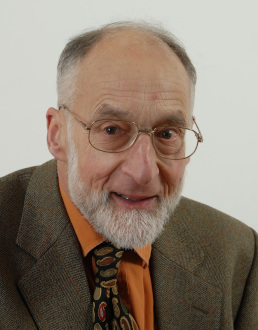
\includegraphics[width=1\textwidth]{milner.jpg}
              \end{figure}
            \end{column}
            \begin{column}{.1\textwidth}
              \includegraphics[width=1\textwidth]{book.jpg}
            \end{column}
            \begin{column}{.1\textwidth}
            \end{column}
          \end{columns}
    \item Based on labeled transition systems (LTS)
    \item \textbf{Weak}: silent computations are abstracted away
  \end{itemize}
    \vspace*{-1ex}
  \pause
  \begin{block}{Weak bisimilarity of operators}
    \begin{itemize}
      \item Labels (actions): read, write, silent ($\tau$)
      \item Weak bisimilarity of operators ($\approx$): LTS + weak simulation + greatest weak bisimulation
      \item $\approx$ has a useful coinduction principle
      \item $\EndOp \approx \SpinOp \approx \SpinOp$ and $\const{ex1} \approx \const{ex2} \approx \const{ex3}$
    \end{itemize}
  \end{block}
  % \begin{block}{intuition}
  %   \footnotesize{two operators are bisimilar if their corresponding transition systems can mutually simulate each other’s transitions.}
  % \end{block}
\end{frame}

% \begin{frame}[fragile]
%   \frametitle{Operators Equivalences: Label Transition System}
%   \begin{tcolorbox}[enhanced,title=Label Transition System,colback=yellow!30]
%     \vspace*{-3ex}
%     \hspace*{-5ex}
%     \begin{align*}
%         &    \cmd{datatype}\ (\tvar{i}, \tvar{o}, \tvar{d})\ \type{IO} = \const{Inp}\ \tvar{i}\ \tvar{d}\ |\ \const{Out}\ \tvar{o}\ \tvar{d}\ |\ \const{Tau}
%         \\[\jot]
%         & \cmd{inductive}\ \const{step}\ \cmd{where}\\
%         & \more \const{step}\ (\const{Inp}\ \var{p}\ \var{x})\ (\const{Read}\ \var{p}\ \var{f})\ (\var{f}\ \var{x}) \\
%         & \bmore \const{step}\ (\const{Out}\ \var{q}\ \var{x})\ (\const{Write}\ \var{op}\ \var{q}\ \var{x})\ \var{op} \\
%         & \bmore \const{step}\ \const{Tau}\ (\const{Silent}\ \var{op})\ \var{op} \\
%         & \bmore \var{op} \in_c \var{ops} \implies \const{step}\ \var{io}\ \var{op}\ \var{op}' \implies \const{step}\ \var{io}\ (\const{Choice}\ \var{ops})\ \var{op}'
%     \end{align*}
%   \end{tcolorbox}
% \end{frame}

% \begin{frame}[fragile]
%   \frametitle{Operators Equivalences: Weak Bisimilarity}
%     \vspace*{-2ex}
%   \begin{tcolorbox}[enhanced,title=Weakly Simulates,colback=yellow!30]
%     \vspace*{-4ex}
%     \hspace*{-5ex}
%     \begin{align*}
%      & \const{estep}\ \const{Tau} = (\const{step}\ \const{Tau})^{==} \\
%      & \const{estep}\ \var{io} = \const{step}\ \var{io}
%     \\
%     &  \const{wstep}\ \var{io} = (\const{step}\ \const{Tau})^{**}\ \const{OO}\ (\const{estep}\ \var{io})\ \const{OO}\ (\const{step}\ \const{Tau})^{**}
%     \\
%     & \const{wsim}\ \var{R}\ \var{op}_1\ \var{op}_2 = (\forall \var{io}\; \var{op}'_1.\ \const{step}\ \var{io}\ \var{op}_1\ \var{op}'_1 \Implies (\exists \var{op}'_2.\ \const{wstep}\ \var{io}\ \var{op}_2\ \var{op}'_2 \land \var{R}\ \var{op}'_1\ \var{op}'_2))
%     \end{align*}
%     \vspace*{-5ex}
%   \end{tcolorbox}
%   \vspace*{-1ex}
%   \begin{itemize}
%     \item A Relation \isabelleinline{\var{R}} is a \emph{weak simulation} if \isabelleinline{\forall \var{op}_1\; \var{op}_2.\ \var{R}\ \var{op}_1\ \var{op}_2 \Implies \const{wsim}\ \var{R}\ \var{op}_1\ \var{op}_2}.
%   \end{itemize}
%     \vspace*{-1.3ex}
%   \pause
%   \begin{tcolorbox}[enhanced,title=Weak Bisimilarity,colback=yellow!30]
%     \vspace*{-3ex}
%     \hspace*{-5ex}
%     \begin{align*}
%      & \cmd{coinductive}\ \const{wbisim}\ (\cmd{infix} \wbisim{}{} 40)\ \cmd{where}\\
%      & \more \const{wsim}\ (\approx)\ \var{op}_1\ \var{op}_2 \implies \const{wsim}\ (\approx)\ \var{op}_2\ \var{op}_1 \implies \wbisim{\var{op}_1}{\var{op}_2}
%     \end{align*}
%     \vspace*{-5ex}
%   \end{tcolorbox}
%   \vspace*{-1ex}
%   \begin{itemize}
%     \item \isabelleinline{\var{R}} is a \emph{weak bisimulation} when both \isabelleinline{\var{R}} and its converse \isabelleinline{\var{R}^{\const{-1}}} are weak simulations. \\
%           Weak bisimilarity is the largest weak bisimulation.
%   \end{itemize}

%   \pause
%   \begin{itemize}
%     \item $\approx$ has a useful coinduction principle
%     \item $\EndOp \approx \SpinOp \approx \SilentOp$ and $\const{ex1} \approx \const{ex2} \approx \const{ex3}$
%   \end{itemize}
% \end{frame}

\section{Asynchronous Dataflow Operators}

\begin{frame}[fragile]
  \frametitle{Auxiliary Definitions}
    \visible<1->{
      \begin{itemize}
        \visible<2->{\item Buffers: $\tvar{p} \Fun \tvar{d}\ list$}
        \visible<3->{\item $\const{choices}$: computes the set of operators that immediately perform next actions}
      \end{itemize}
      }
      \pause
  \begin{tcbraster}[raster columns=2, raster equal height]
      \vspace*{+1ex}
    \begin{tcolorbox}[enhanced,title=Buffer functions,colback=yellow!30]
        \vspace*{-4ex}
      \begin{align*}
        & \hspace*{-6ex} \const{BHD}\ \var{p}\ \var{buf} = \const{hd}\ (\var{buf}\ \var{p})
        \\
        & \hspace*{-6ex} \const{BTL}\ \var{p}\ \var{buf} = \var{buf}(\var{p} := \const{tl}\ (\var{buf}\ \var{p}))
        \\
        & \hspace*{-6ex} \const{BENQ}\ \var{p}\ \var{x}\ \var{buf} = \var{buf}(\var{p} := \var{buf}\ \var{p}\ \const{@}\ [\var{x}])
        % \\
        % & \hspace*{-6ex} \BulkBenq{\var{buf}_1}{\var{buf}_2} = (\lambda \var{p}.\ \var{buf}_2\ \var{p}\ \const{@}\ \var{buf}_1\ \var{p})
      \end{align*}
    \end{tcolorbox}
      \pause
    \begin{tcolorbox}[enhanced,title=choices type,colback=yellow!30]
      \vspace*{-4ex}
      \begin{align*}
        & \hspace*{-6ex} \const{choices} \oftype \type{(\tvar{i}, \tvar{o}, \tvar{d})\ \type{op} \Fun ((\tvar{i}, \tvar{o}, \tvar{d})\ \type{op})\ \type{set}} \\
        % & \hspace*{-6ex} \const{choices}\ \SpinOp = \Emptyset \\
        % & \hspace*{-6ex} \const{Silent}\ \var{op}' \in_c \const{choices}\ \var{op} \Iff \const{step}\ \const{Tau}\ \var{op}\ \var{op}' \\
        % & \hspace*{-6ex} \const{choices}\; (\const{Choice}\ \var{ops}) = \bigcup {}_c \ (\const{choices}\ \Image_c\ \var{ops})
      \end{align*}
      \vspace*{-5ex}
    \end{tcolorbox}
  \end{tcbraster}
      \visible<4->{
      \begin{tcolorbox}[enhanced,title=Mapping ports functions,colback=yellow!30,]
        \vspace*{-4ex}
        \begin{align*}
          & \hspace*{-6ex} \const{map\_op} \oftype \type{(\tvar{i}_1 \Fun \tvar{i}_2) \Fun (\tvar{o}_1 \Fun \tvar{o}_2) \Fun (\tvar{i}_1, \tvar{o}_1, \tvar{d})\ \type{op} \Fun (\tvar{i}_2, \tvar{o}_2, \tvar{d})\ \type{op}} \\
          % & \hspace*{-6ex} \const{projl}\ \oftype \type{(\tvar{a} + \tvar{b}) \Fun \tvar{a}} \\
          % & \hspace*{-6ex} \const{projr}\ \oftype \type{(\tvar{a} + \tvar{b}) \Fun \tvar{b}} \\
          & \hspace*{-6ex} \reassoc\ \oftype \type{(\tvar{a} + \tvar{b}) + \tvar{c} \Fun \tvar{a} + \tvar{b} + \tvar{c}} \\
          & \hspace*{-6ex} \assoc\ \oftype \type{\tvar{a} + \tvar{b} + \tvar{c} \Fun (\tvar{a} + \tvar{b}) + \tvar{c} }
        \end{align*}
        \vspace*{-5ex}
      \end{tcolorbox}
      }
\end{frame}

\begin{frame}[fragile]
  \frametitle{Identity}
  \begin{tcolorbox}[enhanced,title=Equation of the identity operator,colback=yellow!30]
    \vspace*{-3ex}
    \hspace*{-5ex}
    \begin{align*}
      & \const{id_op}\ \var{buf} = \const{Choice}
      \\
      & \visible<2->{(((\lambda \var{p}.\ \const{Read}\ \var{p}\ (\lambda \var{x}.\ \const{id_op}\ (\const{BENQ}\ \var{p}\ \var{x}\ \var{buf})))\ \Image_c \ \Univ_c)\ }
      \\
      &\Union_c
      \\
      &\visible<3->{\phantom{(}((\lambda \var{p}.\ \const{Write}\ (\const{id_op}\ (\const{BTL}\ \var{p}\ \var{buf}))\ \var{p}\ (\const{BHD}\ \var{p}\ \var{buf}))\ \Image_c \ \{\var{p} \in_c \Univ_c \mid \var{buf}\ \var{p} \neq []\}))}
    \end{align*}
  \end{tcolorbox}

  \visible<2->{
    \begin{itemize}
            \visible<2->{\item $\Univ_c$ is the set of usable ports provide by its type}
            \visible<4->{\item Stream delayer: always can read, and it may eventually output}
    \end{itemize}
  }

  \visible<5->{
  \begin{tcolorbox}[enhanced,title=Identity operator with an empty buffer,colback=yellow!30]
    \vspace*{-3ex}
    \hspace*{-5ex}
    \begin{align*}
      \IdOp = \const{id_op}\ (\lambda \_.\ [])
    \end{align*}
  \end{tcolorbox}
  }
\end{frame}

\begin{frame}[fragile]
  \frametitle{Composition: Preliminaries}
  \vspace*{-2ex}
  \begin{tcolorbox}[enhanced,title=Composition operator type,colback=yellow!30]
    \vspace*{-4ex}
    \hspace*{-8ex}
    \begin{align*}
      & \hspace*{-6ex} \const{comp_op}\ \oftype \type{(\tvar{o}_1 \Fun \tvar{i}_2 \ \type{option}) \Fun (\tvar{i}_2 \Fun \tvar{d}\ list) \Fun (\tvar{i}_1, \tvar{o}_1, \tvar{d})\ \type{op} \Fun (\tvar{i}_2, \tvar{o}_2, \tvar{d})\ \type{op} \Fun} \\
      & \hspace*{6.5ex} \type{(\tvar{i}_1 + \tvar{i}_2, \tvar{o}_1 + \tvar{o}_2, \tvar{d})\ \type{op}}
    \end{align*}
    \vspace*{-5ex}
  \end{tcolorbox}
  \pause

  \begin{tcolorbox}[enhanced,title=Sequential and parallel composition,colback=yellow!30]
    \vspace*{-4ex}
    \hspace*{-8ex}
    \begin{align*}
      & \Pcomp{\var{op}_1}{\var{op}_2} = \const{comp_op}\ (\lambda \_.\ \const{None})\ (\lambda \_.\ [])\ \var{op}_1\ \var{op}_2 \\
      & \Scomp{\var{op}_1}{\var{op}_2} = \const{map_op}\ \const{projl}\ \const{projr}\ (\const{comp_op}\ \const{Some}\ (\lambda \_.\ [])\ \var{op}_1\ \var{op}_2)
    \end{align*}
    \vspace*{-5ex}
  \end{tcolorbox}
\end{frame}

\begin{frame}[fragile]
  \frametitle{Composition: Equation}
  \vspace*{-2ex}
  \begin{tcolorbox}[enhanced,title=Equation of the composition operator,colback=yellow!30]
    \vspace*{-4ex}
    \hspace*{-8ex}
    \begin{align*}
     &\visible<1->{\const{comp_op}\ \var{wire}\ \var{buf}\ \var{op}_1\ \var{op}_2 =} \visible<2->{\const{Choice}\ } \visible<4->{(((\lambda \var{op}.\ \syntax{case}\ \var{op}\ \syntax{of}}\\
     &\visible<4->{\more \const{Read}\ \var{p}\ \var{f}\ \Fun \const{Read}\ (\const{Inl}\ \var{p})\ (\lambda x.\ \const{comp_op}\ \var{wire}\ \var{buf}\ (\var{f}\ \var{x})\ \var{op}_2)}\\
     &\visible<5->{\bmore \const{Write}\ \var{op}\ \var{p}\ \var{x} \Fun (\syntax{case}\ \var{wire}\ \var{p}\ \syntax{of}}\\
     &\visible<5->{\more \more \const{None} \Fun \const{Write}\ (\const{comp_op}\ \var{wire}\ \var{buf}\ \var{op}\ \var{op}_2)\ (\const{Inl}\ \var{p})\ \var{x}}\\
     &\visible<5->{\more \bmore \const{Some}\ \var{q} \Fun \const{Silent}\ (\const{comp_op}\ \var{wire}\ (\const{BENQ}\ \var{q}\ \var{x}\ \var{buf})\ \var{op}\ \var{op}_2))}\\
     &\visible<6->{\bmore \const{Silent}\ \var{op} \Fun \const{Silent}\ (\const{comp_op}\ \var{wire}\ \var{buf}\ \var{op}\ \var{op}_2))} \ \visible<3->{\Image_c \ \const{choices}\ \var{op}_1)} \ \visible<2->{\Union_c}\\
     &\visible<9->{\phantom{(}((\lambda \var{op}.\ \syntax{case}\ \var{op}\ \syntax{of}}\\
     &\visible<10->{\more \const{Read}\ \var{p}\ \var{f} \Fun \syntax{if}\ \var{p} \in \const{ran}\ \var{wire}}\\
     &\visible<10->{\more \more \syntax{then}\ \const{Silent}\ (\const{comp_op}\ \var{wire}\ (\const{BTL}\ \var{p}\ \var{buf})\ \var{op}_1\ (\var{f}\ (\const{BHD}\ \var{p}\ \var{buf})))}\\
     &\visible<10->{\more \more \syntax{else}\ \const{Read}\ (\const{Inr}\ \var{p})\ (\lambda \var{x}.\ \const{comp_op}\ \var{wire}\ \var{buf}\ \var{op}_1\ (\var{f}\ \var{x}))}\\
     &\visible<9->{\bmore \const{Write}\ \var{op}\ \var{p}\ \var{x} \Fun \const{Write}\ (\const{comp_op}\ \var{wire}\ \var{buf}\ \var{op}_1\ \var{op})\ (\const{Inr}\ \var{p})\ \var{x}}\\
     &\visible<11->{\bmore \const{Silent}\ \var{op} \Fun \const{Silent}\ (\const{comp_op}\ \var{wire}\ \var{buf}\ \var{op}_1\ \var{op}))} \ \visible<8->{\Image_c \ \const{sound_reads}\ \var{wire}\ \var{buf}\ } \visible<7->{(\const{choices}\ \var{op}_2)))}
    \end{align*}
    \vspace*{-5ex}
  \end{tcolorbox}

\end{frame}

\begin{frame}[fragile]
  \frametitle{Asynchronous Dataflow Operators}
  \begin{itemize}
    \item Identity: $\IdOp$
    \item Parallel composition: $\Pcomp{\var{op}_1}{\var{op}_2}$
    \item Sequential composition: $\Scomp{\var{op}_1}{\var{op}_2}$
  \end{itemize}
  \pause

  \begin{tcbraster}[raster columns=2, raster equal height]
  \begin{tcolorbox}[enhanced,title=Feedback operator type ($\Feedback{op}$) ,colback=yellow!30]
    \vspace*{-7ex}
    \hspace*{-8ex}
    \begin{align*}
      & \hspace*{-6ex} \Feedback{} \ \oftype \type{(\tvar{i} + \tvar{m}, \tvar{o} + \tvar{m}, \tvar{d}) \ op \Fun (\tvar{i}, \tvar{o}, \tvar{d}) \ op}
    \end{align*}
    \vspace*{-6ex}
  \end{tcolorbox}
  \pause
  \begin{tcolorbox}[enhanced,title=Transpose operator type,colback=yellow!30]
    \vspace*{-7ex}
    \hspace*{-8ex}
    \begin{align*}
      & \hspace*{-6ex} \TranspOp \ \oftype \type{(\tvar{n} + \tvar{m}, \tvar{m} + \tvar{n}, \tvar{d}) \ op}
    \end{align*}
    \vspace*{-6ex}
  \end{tcolorbox}
  \end{tcbraster}
  \pause

  \begin{tcbraster}[raster columns=2, raster equal height]
  \begin{tcolorbox}[enhanced,title=Dummy source operator type,colback=yellow!30]
    \vspace*{-7ex}
    \hspace*{-8ex}
    \begin{align*}
      & \hspace*{-6ex} \SourceOp \ \oftype \type{(\tvar{i}, \tvar{o}, \tvar{d}) \ op}
    \end{align*}
    \vspace*{-6ex}
  \end{tcolorbox}
  \pause
  \begin{tcolorbox}[enhanced,title=Sink operator type,colback=yellow!30]
    \vspace*{-7ex}
    \hspace*{-8ex}
    \begin{align*}
      & \hspace*{-6ex} \SinkOp \ \oftype \type{(\tvar{i}, \tvar{o}, \tvar{d}) \ op}
    \end{align*}
    \vspace*{-6ex}
  \end{tcolorbox}
  \end{tcbraster}
  \pause

  \begin{tcbraster}[raster columns=2, raster equal height]
  \begin{tcolorbox}[enhanced,title=Split operator type,colback=yellow!30]
    \vspace*{-7ex}
    \hspace*{-8ex}
    \begin{align*}
      & \hspace*{-6ex} \SplitOp \ \oftype \type{(\tvar{n}, \tvar{n} + \tvar{n}, \tvar{d}) \ op}
    \end{align*}
    \vspace*{-6ex}
  \end{tcolorbox}
  \pause
  \begin{tcolorbox}[enhanced,title=Merge operator type,colback=yellow!30]
    \vspace*{-7ex}
    \hspace*{-8ex}
    \begin{align*}
      & \hspace*{-6ex} \MergeOp \ \oftype \type{(\tvar{n} + \tvar{n}, \tvar{n}, \tvar{d}) \ op}
    \end{align*}
    \vspace*{-6ex}
  \end{tcolorbox}
  \end{tcbraster}
  \pause

  \begin{tcbraster}[raster columns=2, raster equal height]
  \begin{tcolorbox}[enhanced,title=Copy operator type,colback=yellow!30]
    \vspace*{-7ex}
    \hspace*{-8ex}
    \begin{align*}
      & \hspace*{-6ex} \AcopyOp \ \oftype \type{(\tvar{n}, \tvar{n} + \tvar{n}, \tvar{d}) \ op}
    \end{align*}
    \vspace*{-6ex}
  \end{tcolorbox}
  \pause
  \begin{tcolorbox}[enhanced,title=Equality test operator type,colback=yellow!30]
    \vspace*{-7ex}
    \hspace*{-8ex}
    \begin{align*}
      & \hspace*{-6ex} \AeqOp \ \oftype \type{(\tvar{n} + \tvar{n}, \tvar{n}, \tvar{d} \ \type{option}) \ op}
    \end{align*}
    \vspace*{-6ex}
  \end{tcolorbox}
  \end{tcbraster}
\end{frame}

\section{Asynchronous Dataflow Properties}
\begin{frame}[fragile]
  \frametitle{Basic Network Algebra Properties}
    \vspace*{-4ex}
\begin{table}[t]
    \begin{tabular}{ l l }
        \multicolumn{2}{l}{$\text{B1}\!:
            \wbisim{\Pcomp{\var{op}_1}{(\Pcomp{\var{op}_2}{\var{op}_3})}}{\const{map_op}\
                \reassoc\ \reassoc\
                \Pcomp{(\Pcomp{\var{op}_1}{\var{op}_2})}{\var{op}_3}}$} \\
        $\text{B2\_1}\!: \wbisim{\Pcomp{\var{op}}{(\IdOp \oftype
                (\type{0}, \type{0}, \tvar{d})\ \type{op})}}{\const{map_op}\ \const{Inl}\
            \const{Inl}\ \var{op}}$ \\
        $\text{B2\_2}\!: \wbisim{\Pcomp{(\IdOp \oftype (\type{0},
                \type{0}, \tvar{d})\ \type{op})}{\var{op}}}{\const{map_op}\ \const{Inr}\
            \const{Inr}\ \var{op}}$ \\
        \multicolumn{2}{l}{$\text{B3}\!:
            \wbisim{\Scomp{(\Scomp{\var{op}_1}{\var{op}_2})}{\var{op}_3}}{\Scomp{\var{op}_1}{(\Scomp{\var{op}_2}{\var{op}_3})}}$} \\
        $\text{B4\_1}\!: \wbisim{\Scomp{\var{op}\, }{\IdOp}}{\var{op}\,}$ &
        $\text{B4\_2}\!: \wbisim{\Scomp{\IdOp}{\var{op}}}{\var{op}}$ \\
        \multicolumn{2}{l}{$\text{B5}\!:
            \wbisim{\Scomp{(\Pcomp{\var{op}_1}{\var{op}_2})}{(\Pcomp{\var{op}_3}{\var{op}_4})}}{\Pcomp{(\Scomp{\var{op}_1}{\var{op}_3})}{(\Scomp{\var{op}_2}{\var{op}_4})}}$} \\
        $\text{B6}\!: \wbisim{\Pcomp{\IdOp}{\IdOp}}{\IdOp}$ &
        $\text{B7}\!: \wbisim{\Scomp{\TranspOp}{\TranspOp}}{\IdOp}$ \\
        \multicolumn{2}{l}{$\text{B8}\!: \wbisim{(\TranspOp \oftype (\tvar{i} + \type{0},
                \type{0} + \tvar{i}, \tvar{d})\ \type{op})}{\const{map_op}\ \const{id}\
                (\const{case_sum}\ \const{Inr}\ \const{Inl})\ \IdOp}$} \\
        \multicolumn{2}{l}{$\text{B9}\!: \wbisim{\TranspOp}{\Scomp{\const{map_op}\
                    \reassoc\ \reassoc\
                    (\Pcomp{\TranspOp}{\IdOp})}{\const{map_op}\ \const{id}\ \assoc\
                    (\Pcomp{\IdOp}{\TranspOp})}}$} \\
        \multicolumn{2}{l}{$\text{B10}\!: \wbisim{\Scomp{(\Pcomp{\var{op}_1}{\var{op}_2})}{\TranspOp}}{\Scomp{\TranspOp}{(\Pcomp{\var{op}_2}{\var{op}_1 )}}}$} \\
        $\text{F1}\!: \wbisim{\Feedback{\IdOp}}{(\IdOp \oftype
            (\type{0}, \type{0}, \tvar{d})\ \type{op})}$ &
        $\text{F2}\!: \wbisim{\Feedback{\TranspOp}}{\IdOp}$ \\
      \multicolumn{2}{l}{$\text{R1}\!:$\hspace{-0.5em}\begin{tabular}[t]{l} $\wbisim{\Scomp{\var{op}_2}{(\Feedback{\var{op}_1})}}{\Feedback{(\Scomp{(\Pcomp{\var{op}_2}{\IdOp})}{\var{op}_1})}}$
        \end{tabular}} \\
        \multicolumn{2}{l}{$\text{R2}\!:$\hspace{-0.5em}\begin{tabular}[t]{l} $\wbisim{\Scomp{(\Feedback{\var{op}_1})}{\var{op}_2}}{\Feedback{(\Scomp{\var{op}_1}{(\Pcomp{\var{op}_2}{\IdOp})})}}$
        \end{tabular}} \\
        \multicolumn{2}{l}{$\text{R3}\!:$\hspace{-0.5em}\begin{tabular}[t]{l}
                $\wbisim{\Pcomp{\var{op}_1}{(\Feedback{\var{op}_2})}}{\Feedback{(\const{map_op}\
                        \assoc\ \assoc\ (\Pcomp{\var{op}_1}{\var{op}_2}))}}$
        \end{tabular}} \\
        \multicolumn{2}{l}{$\text{R4}\!:$\hspace{-0.5em}\begin{tabular}[t]{l} $\wbisim{\Feedback{(\Scomp{\var{op}_1}{(\Pcomp{\IdOp}{\var{op}_2})})}}{\Feedback{(\Scomp{(\Pcomp{\IdOp}{\var{op}_2})}{\var{op}_1})}}$
        \end{tabular}} \\
        \multicolumn{2}{l}{$\text{R5}\!:$\hspace{-0.5em}\begin{tabular}[t]{l}
                $\wbisim{\const{map_op}\ \const{Inl}\ \const{Inl}\ (\Feedback{(\var{op}  \oftype (\tvar{i} + \type{0},
                        \tvar{o} + \type{0}, \tvar{d})\ \type{op})})}{\var{op}}$
        \end{tabular}} \\
        \multicolumn{2}{l}{$\text{R6}\!:$\hspace{-0.5em}\begin{tabular}[t]{l}
                $\wbisim{\Feedback{(\Feedback{\var{op}})}}{\Feedback{(\const{map_op}\ \reassoc\ \reassoc \ \var{op})}}$
        \end{tabular}}
    \end{tabular}
    \vspace*{-4ex}
\end{table}
\end{frame}

\begin{frame}[fragile, noframenumbering]
  \frametitle{Basic Network Algebra Properties}
    \vspace*{-4ex}
\begin{table}[t]
    \begin{tabular}{ l l }
        \multicolumn{2}{l}{$\text{B1}\!:
            \highlight{\wbisim{\Pcomp{\var{op}_1}{(\Pcomp{\var{op}_2}{\var{op}_3})}}{\const{map_op}\ \reassoc\ \reassoc\ \Pcomp{(\Pcomp{\var{op}_1}{\var{op}_2})}{\var{op}_3}}}$} \\
        $\text{B2\_1}\!: \wbisim{\Pcomp{\var{op}}{(\IdOp \oftype
                (\type{0}, \type{0}, \tvar{d})\ \type{op})}}{\const{map_op}\ \const{Inl}\
            \const{Inl}\ \var{op}}$ \\
        $\text{B2\_2}\!: \wbisim{\Pcomp{(\IdOp \oftype (\type{0},
                \type{0}, \tvar{d})\ \type{op})}{\var{op}}}{\const{map_op}\ \const{Inr}\
            \const{Inr}\ \var{op}}$ \\
        \multicolumn{2}{l}{$\text{B3}\!:
            \wbisim{\Scomp{(\Scomp{\var{op}_1}{\var{op}_2})}{\var{op}_3}}{\Scomp{\var{op}_1}{(\Scomp{\var{op}_2}{\var{op}_3})}}$} \\
        $\text{B4\_1}\!: \wbisim{\Scomp{\var{op}\, }{\IdOp}}{\var{op}\,}$ &
        $\text{B4\_2}\!: \wbisim{\Scomp{\IdOp}{\var{op}}}{\var{op}}$ \\
        \multicolumn{2}{l}{$\text{B5}\!:
            \wbisim{\Scomp{(\Pcomp{\var{op}_1}{\var{op}_2})}{(\Pcomp{\var{op}_3}{\var{op}_4})}}{\Pcomp{(\Scomp{\var{op}_1}{\var{op}_3})}{(\Scomp{\var{op}_2}{\var{op}_4})}}$} \\
        $\text{B6}\!: \wbisim{\Pcomp{\IdOp}{\IdOp}}{\IdOp}$ &
        $\text{B7}\!: \wbisim{\Scomp{\TranspOp}{\TranspOp}}{\IdOp}$ \\
        \multicolumn{2}{l}{$\text{B8}\!: \wbisim{(\TranspOp \oftype (\tvar{i} + \type{0},
                \type{0} + \tvar{i}, \tvar{d})\ \type{op})}{\const{map_op}\ \const{id}\
                (\const{case_sum}\ \const{Inr}\ \const{Inl})\ \IdOp}$} \\
        \multicolumn{2}{l}{$\text{B9}\!: \wbisim{\TranspOp}{\Scomp{\const{map_op}\
                    \reassoc\ \reassoc\
                    (\Pcomp{\TranspOp}{\IdOp})}{\const{map_op}\ \const{id}\ \assoc\
                    (\Pcomp{\IdOp}{\TranspOp})}}$} \\
        \multicolumn{2}{l}{$\text{B10}\!: \wbisim{\Scomp{(\Pcomp{\var{op}_1}{\var{op}_2})}{\TranspOp}}{\Scomp{\TranspOp}{(\Pcomp{\var{op}_2}{\var{op}_1 )}}}$} \\
        $\text{F1}\!: \wbisim{\Feedback{\IdOp}}{(\IdOp \oftype
            (\type{0}, \type{0}, \tvar{d})\ \type{op})}$ &
        $\text{F2}\!: \wbisim{\Feedback{\TranspOp}}{\IdOp}$ \\
      \multicolumn{2}{l}{$\text{R1}\!:$\hspace{-0.5em}\begin{tabular}[t]{l} $\wbisim{\Scomp{\var{op}_2}{(\Feedback{\var{op}_1})}}{\Feedback{(\Scomp{(\Pcomp{\var{op}_2}{\IdOp})}{\var{op}_1})}}$
        \end{tabular}} \\
        \multicolumn{2}{l}{$\text{R2}\!:$\hspace{-0.5em}\begin{tabular}[t]{l} $\wbisim{\Scomp{(\Feedback{\var{op}_1})}{\var{op}_2}}{\Feedback{(\Scomp{\var{op}_1}{(\Pcomp{\var{op}_2}{\IdOp})})}}$
        \end{tabular}} \\
        \multicolumn{2}{l}{$\text{R3}\!:$\hspace{-0.5em}\begin{tabular}[t]{l}
                $\wbisim{\Pcomp{\var{op}_1}{(\Feedback{\var{op}_2})}}{\Feedback{(\const{map_op}\
                        \assoc\ \assoc\ (\Pcomp{\var{op}_1}{\var{op}_2}))}}$
        \end{tabular}} \\
        \multicolumn{2}{l}{$\text{R4}\!:$\hspace{-0.5em}\begin{tabular}[t]{l} $\wbisim{\Feedback{(\Scomp{\var{op}_1}{(\Pcomp{\IdOp}{\var{op}_2})})}}{\Feedback{(\Scomp{(\Pcomp{\IdOp}{\var{op}_2})}{\var{op}_1})}}$
        \end{tabular}} \\
        \multicolumn{2}{l}{$\text{R5}\!:$\hspace{-0.5em}\begin{tabular}[t]{l}
                $\wbisim{\const{map_op}\ \const{Inl}\ \const{Inl}\ (\Feedback{(\var{op}  \oftype (\tvar{i} + \type{0},
                        \tvar{o} + \type{0}, \tvar{d})\ \type{op})})}{\var{op}}$
        \end{tabular}} \\
        \multicolumn{2}{l}{$\text{R6}\!:$\hspace{-0.5em}\begin{tabular}[t]{l}
                $\wbisim{\Feedback{(\Feedback{\var{op}})}}{\Feedback{(\const{map_op}\ \reassoc\ \reassoc \ \var{op})}}$
        \end{tabular}}
    \end{tabular}
    \vspace*{-4ex}
\end{table}
\end{frame}

\begin{frame}[fragile, noframenumbering]
  \frametitle{Basic Network Algebra Properties}
    \vspace*{-4ex}
\begin{table}[t]
    \begin{tabular}{ l l }
        \multicolumn{2}{l}{$\text{B1}\!:
            \wbisim{\Pcomp{\var{op}_1}{(\Pcomp{\var{op}_2}{\var{op}_3})}}{\const{map_op}\ \reassoc\ \reassoc\ \Pcomp{(\Pcomp{\var{op}_1}{\var{op}_2})}{\var{op}_3}}$} \\
        $\text{B2\_1}\!: \wbisim{\Pcomp{\var{op}}{(\IdOp \oftype
                (\type{0}, \type{0}, \tvar{d})\ \type{op})}}{\const{map_op}\ \const{Inl}\
            \const{Inl}\ \var{op}}$ \\
        $\text{B2\_2}\!: \wbisim{\Pcomp{(\IdOp \oftype (\type{0},
                \type{0}, \tvar{d})\ \type{op})}{\var{op}}}{\const{map_op}\ \const{Inr}\
            \const{Inr}\ \var{op}}$ \\
        \multicolumn{2}{l}{$\text{B3}\!:
            \highlight{\wbisim{\Scomp{(\Scomp{\var{op}_1}{\var{op}_2})}{\var{op}_3}}{\Scomp{\var{op}_1}{(\Scomp{\var{op}_2}{\var{op}_3})}}}$} \\
        $\text{B4\_1}\!: \wbisim{\Scomp{\var{op}\, }{\IdOp}}{\var{op}\,}$ &
        $\text{B4\_2}\!: \wbisim{\Scomp{\IdOp}{\var{op}}}{\var{op}}$ \\
        \multicolumn{2}{l}{$\text{B5}\!:
            \wbisim{\Scomp{(\Pcomp{\var{op}_1}{\var{op}_2})}{(\Pcomp{\var{op}_3}{\var{op}_4})}}{\Pcomp{(\Scomp{\var{op}_1}{\var{op}_3})}{(\Scomp{\var{op}_2}{\var{op}_4})}}$} \\
        $\text{B6}\!: \wbisim{\Pcomp{\IdOp}{\IdOp}}{\IdOp}$ &
        $\text{B7}\!: \wbisim{\Scomp{\TranspOp}{\TranspOp}}{\IdOp}$ \\
        \multicolumn{2}{l}{$\text{B8}\!: \wbisim{(\TranspOp \oftype (\tvar{i} + \type{0},
                \type{0} + \tvar{i}, \tvar{d})\ \type{op})}{\const{map_op}\ \const{id}\
                (\const{case_sum}\ \const{Inr}\ \const{Inl})\ \IdOp}$} \\
        \multicolumn{2}{l}{$\text{B9}\!: \wbisim{\TranspOp}{\Scomp{\const{map_op}\
                    \reassoc\ \reassoc\
                    (\Pcomp{\TranspOp}{\IdOp})}{\const{map_op}\ \const{id}\ \assoc\
                    (\Pcomp{\IdOp}{\TranspOp})}}$} \\
        \multicolumn{2}{l}{$\text{B10}\!: \wbisim{\Scomp{(\Pcomp{\var{op}_1}{\var{op}_2})}{\TranspOp}}{\Scomp{\TranspOp}{(\Pcomp{\var{op}_2}{\var{op}_1 )}}}$} \\
        $\text{F1}\!: \wbisim{\Feedback{\IdOp}}{(\IdOp \oftype
            (\type{0}, \type{0}, \tvar{d})\ \type{op})}$ &
        $\text{F2}\!: \wbisim{\Feedback{\TranspOp}}{\IdOp}$ \\
      \multicolumn{2}{l}{$\text{R1}\!:$\hspace{-0.5em}\begin{tabular}[t]{l} $\wbisim{\Scomp{\var{op}_2}{(\Feedback{\var{op}_1})}}{\Feedback{(\Scomp{(\Pcomp{\var{op}_2}{\IdOp})}{\var{op}_1})}}$
        \end{tabular}} \\
        \multicolumn{2}{l}{$\text{R2}\!:$\hspace{-0.5em}\begin{tabular}[t]{l} $\wbisim{\Scomp{(\Feedback{\var{op}_1})}{\var{op}_2}}{\Feedback{(\Scomp{\var{op}_1}{(\Pcomp{\var{op}_2}{\IdOp})})}}$
        \end{tabular}} \\
        \multicolumn{2}{l}{$\text{R3}\!:$\hspace{-0.5em}\begin{tabular}[t]{l}
                $\wbisim{\Pcomp{\var{op}_1}{(\Feedback{\var{op}_2})}}{\Feedback{(\const{map_op}\
                        \assoc\ \assoc\ (\Pcomp{\var{op}_1}{\var{op}_2}))}}$
        \end{tabular}} \\
        \multicolumn{2}{l}{$\text{R4}\!:$\hspace{-0.5em}\begin{tabular}[t]{l} $\wbisim{\Feedback{(\Scomp{\var{op}_1}{(\Pcomp{\IdOp}{\var{op}_2})})}}{\Feedback{(\Scomp{(\Pcomp{\IdOp}{\var{op}_2})}{\var{op}_1})}}$
        \end{tabular}} \\
        \multicolumn{2}{l}{$\text{R5}\!:$\hspace{-0.5em}\begin{tabular}[t]{l}
                $\wbisim{\const{map_op}\ \const{Inl}\ \const{Inl}\ (\Feedback{(\var{op}  \oftype (\tvar{i} + \type{0},
                        \tvar{o} + \type{0}, \tvar{d})\ \type{op})})}{\var{op}}$
        \end{tabular}} \\
        \multicolumn{2}{l}{$\text{R6}\!:$\hspace{-0.5em}\begin{tabular}[t]{l}
                $\wbisim{\Feedback{(\Feedback{\var{op}})}}{\Feedback{(\const{map_op}\ \reassoc\ \reassoc \ \var{op})}}$
        \end{tabular}}
    \end{tabular}
    \vspace*{-4ex}
\end{table}
\end{frame}

\begin{frame}[fragile, noframenumbering]
  \frametitle{Basic Network Algebra Properties}
    \vspace*{-4ex}
\begin{table}[t]
    \begin{tabular}{ l l }
        \multicolumn{2}{l}{$\text{B1}\!:
            \wbisim{\Pcomp{\var{op}_1}{(\Pcomp{\var{op}_2}{\var{op}_3})}}{\const{map_op}\ \reassoc\ \reassoc\ \Pcomp{(\Pcomp{\var{op}_1}{\var{op}_2})}{\var{op}_3}}$} \\
        $\text{B2\_1}\!: \wbisim{\Pcomp{\var{op}}{(\IdOp \oftype
                (\type{0}, \type{0}, \tvar{d})\ \type{op})}}{\const{map_op}\ \const{Inl}\
            \const{Inl}\ \var{op}}$ \\
        $\text{B2\_2}\!: \wbisim{\Pcomp{(\IdOp \oftype (\type{0},
                \type{0}, \tvar{d})\ \type{op})}{\var{op}}}{\const{map_op}\ \const{Inr}\
            \const{Inr}\ \var{op}}$ \\
        \multicolumn{2}{l}{$\text{B3}\!:
            \wbisim{\Scomp{(\Scomp{\var{op}_1}{\var{op}_2})}{\var{op}_3}}{\Scomp{\var{op}_1}{(\Scomp{\var{op}_2}{\var{op}_3})}}$} \\
        $\text{B4\_1}\!: \wbisim{\Scomp{\var{op}\, }{\IdOp}}{\var{op}\,}$ &
        $\text{B4\_2}\!: \wbisim{\Scomp{\IdOp}{\var{op}}}{\var{op}}$ \\
        \multicolumn{2}{l}{$\text{B5}\!:
            \wbisim{\Scomp{(\Pcomp{\var{op}_1}{\var{op}_2})}{(\Pcomp{\var{op}_3}{\var{op}_4})}}{\Pcomp{(\Scomp{\var{op}_1}{\var{op}_3})}{(\Scomp{\var{op}_2}{\var{op}_4})}}$} \\
        $\text{B6}\!: \wbisim{\Pcomp{\IdOp}{\IdOp}}{\IdOp}$ &
        $\text{B7}\!: \wbisim{\Scomp{\TranspOp}{\TranspOp}}{\IdOp}$ \\
        \multicolumn{2}{l}{$\text{B8}\!: \wbisim{(\TranspOp \oftype (\tvar{i} + \type{0},
                \type{0} + \tvar{i}, \tvar{d})\ \type{op})}{\const{map_op}\ \const{id}\
                (\const{case_sum}\ \const{Inr}\ \const{Inl})\ \IdOp}$} \\
        \multicolumn{2}{l}{$\text{B9}\!: \wbisim{\TranspOp}{\Scomp{\const{map_op}\
                    \reassoc\ \reassoc\
                    (\Pcomp{\TranspOp}{\IdOp})}{\const{map_op}\ \const{id}\ \assoc\
                    (\Pcomp{\IdOp}{\TranspOp})}}$} \\
        \multicolumn{2}{l}{$\text{B10}\!: \highlight{\wbisim{\Scomp{(\Pcomp{\var{op}_1}{\var{op}_2})}{\TranspOp}}{\Scomp{\TranspOp}{(\Pcomp{\var{op}_2}{\var{op}_1 )}}}}$} \\
        $\text{F1}\!: \wbisim{\Feedback{\IdOp}}{(\IdOp \oftype
            (\type{0}, \type{0}, \tvar{d})\ \type{op})}$ &
        $\text{F2}\!: \wbisim{\Feedback{\TranspOp}}{\IdOp}$ \\
      \multicolumn{2}{l}{$\text{R1}\!:$\hspace{-0.5em}\begin{tabular}[t]{l} $\wbisim{\Scomp{\var{op}_2}{(\Feedback{\var{op}_1})}}{\Feedback{(\Scomp{(\Pcomp{\var{op}_2}{\IdOp})}{\var{op}_1})}}$
        \end{tabular}} \\
        \multicolumn{2}{l}{$\text{R2}\!:$\hspace{-0.5em}\begin{tabular}[t]{l} $\wbisim{\Scomp{(\Feedback{\var{op}_1})}{\var{op}_2}}{\Feedback{(\Scomp{\var{op}_1}{(\Pcomp{\var{op}_2}{\IdOp})})}}$
        \end{tabular}} \\
        \multicolumn{2}{l}{$\text{R3}\!:$\hspace{-0.5em}\begin{tabular}[t]{l}
                $\wbisim{\Pcomp{\var{op}_1}{(\Feedback{\var{op}_2})}}{\Feedback{(\const{map_op}\
                        \assoc\ \assoc\ (\Pcomp{\var{op}_1}{\var{op}_2}))}}$
        \end{tabular}} \\
        \multicolumn{2}{l}{$\text{R4}\!:$\hspace{-0.5em}\begin{tabular}[t]{l} $\wbisim{\Feedback{(\Scomp{\var{op}_1}{(\Pcomp{\IdOp}{\var{op}_2})})}}{\Feedback{(\Scomp{(\Pcomp{\IdOp}{\var{op}_2})}{\var{op}_1})}}$
        \end{tabular}} \\
        \multicolumn{2}{l}{$\text{R5}\!:$\hspace{-0.5em}\begin{tabular}[t]{l}
                $\wbisim{\const{map_op}\ \const{Inl}\ \const{Inl}\ (\Feedback{(\var{op}  \oftype (\tvar{i} + \type{0},
                        \tvar{o} + \type{0}, \tvar{d})\ \type{op})})}{\var{op}}$
        \end{tabular}} \\
        \multicolumn{2}{l}{$\text{R6}\!:$\hspace{-0.5em}\begin{tabular}[t]{l}
                $\wbisim{\Feedback{(\Feedback{\var{op}})}}{\Feedback{(\const{map_op}\ \reassoc\ \reassoc \ \var{op})}}$
        \end{tabular}}
    \end{tabular}
    \vspace*{-4ex}
\end{table}
\end{frame}

\begin{frame}[fragile, noframenumbering]
  \frametitle{Basic Network Algebra Properties}
    \vspace*{-4ex}
\begin{table}[t]
    \begin{tabular}{ l l }
        \multicolumn{2}{l}{$\text{B1}\!:
            \wbisim{\Pcomp{\var{op}_1}{(\Pcomp{\var{op}_2}{\var{op}_3})}}{\const{map_op}\ \reassoc\ \reassoc\ \Pcomp{(\Pcomp{\var{op}_1}{\var{op}_2})}{\var{op}_3}}$} \\
        $\text{B2\_1}\!: \wbisim{\Pcomp{\var{op}}{(\IdOp \oftype
                (\type{0}, \type{0}, \tvar{d})\ \type{op})}}{\const{map_op}\ \const{Inl}\
            \const{Inl}\ \var{op}}$ \\
        $\text{B2\_2}\!: \wbisim{\Pcomp{(\IdOp \oftype (\type{0},
                \type{0}, \tvar{d})\ \type{op})}{\var{op}}}{\const{map_op}\ \const{Inr}\
            \const{Inr}\ \var{op}}$ \\
        \multicolumn{2}{l}{$\text{B3}\!:
            \wbisim{\Scomp{(\Scomp{\var{op}_1}{\var{op}_2})}{\var{op}_3}}{\Scomp{\var{op}_1}{(\Scomp{\var{op}_2}{\var{op}_3})}}$} \\
        $\text{B4\_1}\!: \wbisim{\Scomp{\var{op}\, }{\IdOp}}{\var{op}\,}$ &
        $\text{B4\_2}\!: \wbisim{\Scomp{\IdOp}{\var{op}}}{\var{op}}$ \\
        \multicolumn{2}{l}{$\text{B5}\!:
            \wbisim{\Scomp{(\Pcomp{\var{op}_1}{\var{op}_2})}{(\Pcomp{\var{op}_3}{\var{op}_4})}}{\Pcomp{(\Scomp{\var{op}_1}{\var{op}_3})}{(\Scomp{\var{op}_2}{\var{op}_4})}}$} \\
        $\text{B6}\!: \wbisim{\Pcomp{\IdOp}{\IdOp}}{\IdOp}$ &
        $\text{B7}\!: \wbisim{\Scomp{\TranspOp}{\TranspOp}}{\IdOp}$ \\
        \multicolumn{2}{l}{$\text{B8}\!: \wbisim{(\TranspOp \oftype (\tvar{i} + \type{0},
                \type{0} + \tvar{i}, \tvar{d})\ \type{op})}{\const{map_op}\ \const{id}\
                (\const{case_sum}\ \const{Inr}\ \const{Inl})\ \IdOp}$} \\
        \multicolumn{2}{l}{$\text{B9}\!: \wbisim{\TranspOp}{\Scomp{\const{map_op}\
                    \reassoc\ \reassoc\
                    (\Pcomp{\TranspOp}{\IdOp})}{\const{map_op}\ \const{id}\ \assoc\
                    (\Pcomp{\IdOp}{\TranspOp})}}$} \\
        \multicolumn{2}{l}{$\text{B10}\!: \wbisim{\Scomp{(\Pcomp{\var{op}_1}{\var{op}_2})}{\TranspOp}}{\Scomp{\TranspOp}{(\Pcomp{\var{op}_2}{\var{op}_1 )}}}$} \\
        $\text{F1}\!: \wbisim{\Feedback{\IdOp}}{(\IdOp \oftype
            (\type{0}, \type{0}, \tvar{d})\ \type{op})}$ &
        $\text{F2}\!: \wbisim{\Feedback{\TranspOp}}{\IdOp}$ \\
      \multicolumn{2}{l}{$\text{R1}\!:$\hspace{-0.5em}\begin{tabular}[t]{l} $\wbisim{\Scomp{\var{op}_2}{(\Feedback{\var{op}_1})}}{\Feedback{(\Scomp{(\Pcomp{\var{op}_2}{\IdOp})}{\var{op}_1})}}$
        \end{tabular}} \\
        \multicolumn{2}{l}{$\text{R2}\!:$\hspace{-0.5em}\begin{tabular}[t]{l} $\wbisim{\Scomp{(\Feedback{\var{op}_1})}{\var{op}_2}}{\Feedback{(\Scomp{\var{op}_1}{(\Pcomp{\var{op}_2}{\IdOp})})}}$
        \end{tabular}} \\
        \multicolumn{2}{l}{$\text{R3}\!:$\hspace{-0.5em}\begin{tabular}[t]{l}
                $\wbisim{\Pcomp{\var{op}_1}{(\Feedback{\var{op}_2})}}{\Feedback{(\const{map_op}\
                        \assoc\ \assoc\ (\Pcomp{\var{op}_1}{\var{op}_2}))}}$
        \end{tabular}} \\
        \multicolumn{2}{l}{$\text{R4}\!:$\hspace{-0.5em}\begin{tabular}[t]{l} $\wbisim{\Feedback{(\Scomp{\var{op}_1}{(\Pcomp{\IdOp}{\var{op}_2})})}}{\Feedback{(\Scomp{(\Pcomp{\IdOp}{\var{op}_2})}{\var{op}_1})}}$
        \end{tabular}} \\
        \multicolumn{2}{l}{$\text{R5}\!:$\hspace{-0.5em}\begin{tabular}[t]{l}
                $\wbisim{\const{map_op}\ \const{Inl}\ \const{Inl}\ (\Feedback{(\var{op}  \oftype (\tvar{i} + \type{0},
                        \tvar{o} + \type{0}, \tvar{d})\ \type{op})})}{\var{op}}$
        \end{tabular}} \\
        \multicolumn{2}{l}{$\text{R6}\!:$\hspace{-0.5em}\begin{tabular}[t]{l}
                $\highlight{\wbisim{\Feedback{(\Feedback{\var{op}})}}{\Feedback{(\const{map_op}\ \reassoc\ \reassoc \ \var{op})}}}$
        \end{tabular}}
    \end{tabular}
    \vspace*{-4ex}
\end{table}
\end{frame}

\begin{frame}[fragile, noframenumbering]
  \frametitle{Basic Network Algebra Properties}
    \vspace*{-4ex}
\begin{table}[t]
    \begin{tabular}{ l l }
        \multicolumn{2}{l}{$\text{B1}\!:
            \wbisim{\Pcomp{\var{op}_1}{(\Pcomp{\var{op}_2}{\var{op}_3})}}{\const{map_op}\ \reassoc\ \reassoc\ \Pcomp{(\Pcomp{\var{op}_1}{\var{op}_2})}{\var{op}_3}}$} \\
        $\text{B2\_1}\!: \wbisim{\Pcomp{\var{op}}{(\IdOp \oftype
                (\type{0}, \type{0}, \tvar{d})\ \type{op})}}{\const{map_op}\ \const{Inl}\
            \const{Inl}\ \var{op}}$ \\
        $\text{B2\_2}\!: \wbisim{\Pcomp{(\IdOp \oftype (\type{0},
                \type{0}, \tvar{d})\ \type{op})}{\var{op}}}{\const{map_op}\ \const{Inr}\
            \const{Inr}\ \var{op}}$ \\
        \multicolumn{2}{l}{$\text{B3}\!:
            \wbisim{\Scomp{(\Scomp{\var{op}_1}{\var{op}_2})}{\var{op}_3}}{\Scomp{\var{op}_1}{(\Scomp{\var{op}_2}{\var{op}_3})}}$} \\
        $\text{B4\_1}\!: \wbisim{\Scomp{\var{op}\, }{\IdOp}}{\var{op}\,}$ &
        $\text{B4\_2}\!: \wbisim{\Scomp{\IdOp}{\var{op}}}{\var{op}}$ \\
        \multicolumn{2}{l}{$\text{B5}\!:
            \wbisim{\Scomp{(\Pcomp{\var{op}_1}{\var{op}_2})}{(\Pcomp{\var{op}_3}{\var{op}_4})}}{\Pcomp{(\Scomp{\var{op}_1}{\var{op}_3})}{(\Scomp{\var{op}_2}{\var{op}_4})}}$} \\
        $\text{B6}\!: \wbisim{\Pcomp{\IdOp}{\IdOp}}{\IdOp}$ &
        $\text{B7}\!: \wbisim{\Scomp{\TranspOp}{\TranspOp}}{\IdOp}$ \\
        \multicolumn{2}{l}{$\text{B8}\!: \wbisim{(\TranspOp \oftype (\tvar{i} + \type{0},
                \type{0} + \tvar{i}, \tvar{d})\ \type{op})}{\const{map_op}\ \const{id}\
                (\const{case_sum}\ \const{Inr}\ \const{Inl})\ \IdOp}$} \\
        \multicolumn{2}{l}{$\text{B9}\!: \wbisim{\TranspOp}{\Scomp{\const{map_op}\
                    \reassoc\ \reassoc\
                    (\Pcomp{\TranspOp}{\IdOp})}{\const{map_op}\ \const{id}\ \assoc\
                    (\Pcomp{\IdOp}{\TranspOp})}}$} \\
        \multicolumn{2}{l}{$\text{B10}\!: \wbisim{\Scomp{(\Pcomp{\var{op}_1}{\var{op}_2})}{\TranspOp}}{\Scomp{\TranspOp}{(\Pcomp{\var{op}_2}{\var{op}_1 )}}}$} \\
        $\text{F1}\!: \wbisim{\Feedback{\IdOp}}{(\IdOp \oftype
            (\type{0}, \type{0}, \tvar{d})\ \type{op})}$ &
        $\text{F2}\!: \wbisim{\Feedback{\TranspOp}}{\IdOp}$ \\
      \multicolumn{2}{l}{$\text{R1}\!:$\hspace{-0.5em}\begin{tabular}[t]{l} $\wbisim{\Scomp{\var{op}_2}{(\Feedback{\var{op}_1})}}{\Feedback{(\Scomp{(\Pcomp{\var{op}_2}{\IdOp})}{\var{op}_1})}}$
        \end{tabular}} \\
        \multicolumn{2}{l}{$\text{R2}\!:$\hspace{-0.5em}\begin{tabular}[t]{l} $\wbisim{\Scomp{(\Feedback{\var{op}_1})}{\var{op}_2}}{\Feedback{(\Scomp{\var{op}_1}{(\Pcomp{\var{op}_2}{\IdOp})})}}$
        \end{tabular}} \\
        \multicolumn{2}{l}{$\text{R3}\!:$\hspace{-0.5em}\begin{tabular}[t]{l}
                $\wbisim{\Pcomp{\var{op}_1}{(\Feedback{\var{op}_2})}}{\Feedback{(\const{map_op}\
                        \assoc\ \assoc\ (\Pcomp{\var{op}_1}{\var{op}_2}))}}$
        \end{tabular}} \\
        \multicolumn{2}{l}{$\text{R4}\!:$\hspace{-0.5em}\begin{tabular}[t]{l} $\wbisim{\Feedback{(\Scomp{\var{op}_1}{(\Pcomp{\IdOp}{\var{op}_2})})}}{\Feedback{(\Scomp{(\Pcomp{\IdOp}{\var{op}_2})}{\var{op}_1})}}$
        \end{tabular}} \\
        \multicolumn{2}{l}{$\text{R5}\!:$\hspace{-0.5em}\begin{tabular}[t]{l}
                $\highlight{\wbisim{\const{map_op}\ \const{Inl}\ \const{Inl}\ (\Feedback{(\var{op}  \oftype (\tvar{i} + \type{0}, \tvar{o} + \type{0}, \tvar{d})\ \type{op})})}{\var{op}}}$
        \end{tabular}} \\
        \multicolumn{2}{l}{$\text{R6}\!:$\hspace{-0.5em}\begin{tabular}[t]{l}
                $\wbisim{\Feedback{(\Feedback{\var{op}})}}{\Feedback{(\const{map_op}\ \reassoc\ \reassoc \ \var{op})}}$
        \end{tabular}}
    \end{tabular}
    \vspace*{-4ex}
\end{table}
\end{frame}

\begin{frame}[fragile]
  \frametitle{Properties of Equality Test, Merge, Copy, Split, Source and Sink operators}
    \vspace*{-4ex}
\begin{table}[t]
    \addtolength{\tabcolsep}{-0.8em}
    \begin{tabular}{ l l l }
        \multicolumn{3}{l}{$
            \text{A1}\!: \wbisim{\Scomp{(\Pcomp{\AeqOp}{\IdOp})}{\AeqOp}}{\const{map_op}\
                \assoc\ \const{id}\ (\Scomp{(\Pcomp{\IdOp}{\AeqOp})}{\AeqOp})} %\quad \text{for
                %} \ogt \in \{\AeqOp, \MergeOp\}
            $} \\
        $
        \text{A2}\!: \wbisim{\Scomp{\TranspOp}{\ogt}}{\ogt} \quad \text{for } \ogt
        \in \{\AeqOp, \MergeOp\}
        $ &
        $
        \text{A6}\!: \wbisim{\Scomp{\olt}{\TranspOp}}{\olt} \quad \text{for } \olt
        \in \{\AcopyOp, \SplitOp\}
        $ \\
        \multicolumn{3}{l}{$
            \text{A3}_\AeqOp\!: \wbisim{\Scomp{(\Pcomp{(\SourceOp \oftype (\type{0},
                        \tvar{a}, \tvar{d})\ \type{op})}{\IdOp})}{\AeqOp}}{\Scomp{(\SinkOp \oftype
                    (\type{0} + \tvar{a}, \type{0}, \tvar{d})\ \type{op})}{\SourceOp}}
            $} \\
        \multicolumn{3}{l}{$
            \text{A3}_\MergeOp\!: \wbisim{\Scomp{(\Pcomp{(\SourceOp \oftype (\type{0},
                        \tvar{a}, \tvar{d})\ \type{op})}{\IdOp})}{\MergeOp}}{\const{map_op}\
                \const{Inr}\ \const{id}\ \IdOp}
            $} \\
        $
        \text{A4}\!: \wbisim{\Scomp{\ogt}{\SinkOp}}{\Pcomp{\SinkOp}{\SinkOp}}
        \quad \text{for } \ogt \in \{\AeqOp, \MergeOp\}
        $ &
        $
        \text{A8}\!:
        \wbisim{\Scomp{\SourceOp}{\olt}}{\Pcomp{\SourceOp}{\SourceOp}} \quad
        \text{for } \olt \in \{\AcopyOp, \SplitOp\}
        $ \\
        $
        \text{A5}\!:
        \wbisim{\Scomp{\AcopyOp}{(\Pcomp{\AcopyOp}{\IdOp})}}{\const{map_op}\
            \const{id}\ \assoc\ (\Scomp{\AcopyOp}{(\Pcomp{\IdOp}{\AcopyOp})})}
        $ \\
        $
        \text{A7}\!:
        \wbisim{\Scomp{\AcopyOp}{(\Pcomp{\SinkOp}{\IdOp})}}{\const{map_op}\
            \const{id}\ \const{Inr}\ \IdOp}
        $ &
        $
        \text{A9}\!: \wbisim{\Scomp{\SourceOp}{\SinkOp}}{\IdOp}
        $ \\
        \multicolumn{3}{l}{$
            \text{A10}\!:
            \wbisim{\Scomp{\AeqOp}{\AcopyOp}}{\Scomp{\Scomp{(\Pcomp{\AcopyOp}{\AcopyOp})}{(\const{map_op}\
                        \reassoc\ \reassoc\ (\Pcomp{\const{map_op}\ \assoc\ \assoc\
                            (\Pcomp{\IdOp}{\TranspOp})}{\IdOp}))}}{(\Pcomp{\AeqOp\,}{\AeqOp\,})}}
            $} \\
        $
        \text{A11}\!: \wbisim{\Scomp{\AcopyOp}{\AeqOp}}{\IdOp}
        $ &
        $
        \text{A12}\!: \wbisim{\SourceOp}{(\IdOp \oftype (\type{0}, \type{0},
            \tvar{d})\ \type{op})}
        $ \\
        $
        \text{A16}\!: \wbisim{\SinkOp}{(\IdOp \oftype (\type{0}, \type{0},
            \tvar{d})\ \type{op})}
        $ &
        $
        \text{A13}\!: \wbisim{\SourceOp}{\Pcomp{\SourceOp}{\SourceOp}}
        $ &
        $
        \text{A17}\!: \wbisim{\SinkOp}{\Pcomp{\SinkOp}{\SinkOp}}
        $ \\
        \multicolumn{3}{l}{$
            \text{A14}\!: \wbisim{\const{map_op}\ \const{id}\ \const{Inl}\ (\ogt
                \oftype (\type{0} + \type{0}, \type{0}, \tvar{d})\ \type{op})}{\IdOp}
            \quad \text{for } \ogt \in \{\AeqOp, \MergeOp\}
            $} \\
        \multicolumn{3}{l}{$
            \text{A15}\!: \wbisim{\ogt}{\Scomp{\const{map_op}\ \reassoc\ \reassoc\
                    (\Pcomp{\const{map_op}\ \assoc\ \assoc\
                        (\Pcomp{\IdOp}{\TranspOp})}{\IdOp})}{(\Pcomp{\ogt}{\ogt})}} \quad
            \text{for } \ogt \in \{\AeqOp, \MergeOp\}
            $} \\
        \multicolumn{3}{l}{$
            \text{A18}\!: \wbisim{\const{map_op}\ \const{Inl}\ \const{id}\ (\olt
                \oftype (\type{0}, \type{0} + \type{0}, \tvar{d})\ \type{op})}{\IdOp}
            \quad \text{for } \olt \in \{\AcopyOp, \SplitOp\}
            $} \\
        \multicolumn{3}{l}{$
            \text{A19}\!: \wbisim{\olt}{\Scomp{(\Pcomp{\olt}{\olt})}{\const{map_op}\
                    \reassoc\ \reassoc\ (\Pcomp{\const{map_op}\ \assoc\ \assoc\
                        (\Pcomp{\IdOp}{\TranspOp})}{\IdOp})}} \quad \text{for } \olt \in
            \{\AcopyOp, \SplitOp\}
            $} \\
        \multicolumn{3}{l}{$
            \text{F3}\!: \wbisim{\Feedback{(\const{map_op}\ \const{id}\ \const{Inr}\
                    \ogt)}}{\SinkOp} \quad \text{for } \ogt \in \{\AeqOp, \MergeOp\}
            $} \\
        \multicolumn{3}{l}{$
            \text{F4}\!: \wbisim{\Feedback{(\const{map_op}\ \const{Inr}\ \const{id}\
                    \olt)}}{\SourceOp} \quad \text{for } \olt \in \{\AcopyOp, \SplitOp\}
            $} \\
        \multicolumn{3}{l}{$
            \text{F5}\!:
            \wbisim{\Feedback{(\Scomp{\Scomp{(\Pcomp{\IdOp}{\AcopyOp})}{\const{map_op}\
                            \reassoc\ \reassoc\
                            (\Pcomp{\TranspOp}{\IdOp})}}{(\Pcomp{\IdOp}{\AeqOp})})}}{\Scomp{\SinkOp}{\SourceOp}}
            $}
    \end{tabular}
    \vspace*{-4ex}
\end{table}
\end{frame}

\begin{frame}[fragile, noframenumbering]
  \frametitle{Properties of Equality Test, Merge, Copy, Split, Source and Sink operators}
    \vspace*{-4ex}
\begin{table}[t]
    \addtolength{\tabcolsep}{-0.8em}
    \begin{tabular}{ l l l }
        \multicolumn{3}{l}{$\text{A1}\!: \highlight{\wbisim{\Scomp{(\Pcomp{\AeqOp}{\IdOp})}{\AeqOp}}{\const{map_op}\ \assoc\ \const{id}\ (\Scomp{(\Pcomp{\IdOp}{\AeqOp})}{\AeqOp})} %\quad \text{for
                %} \ogt \in \{\AeqOp, \MergeOp\}
            }$} \\
        $
        \text{A2}\!: \wbisim{\Scomp{\TranspOp}{\ogt}}{\ogt} \quad \text{for } \ogt
        \in \{\AeqOp, \MergeOp\}
        $ &
        $
        \text{A6}\!: \wbisim{\Scomp{\olt}{\TranspOp}}{\olt} \quad \text{for } \olt
        \in \{\AcopyOp, \SplitOp\}
        $ \\
        \multicolumn{3}{l}{$
            \text{A3}_\AeqOp\!: \wbisim{\Scomp{(\Pcomp{(\SourceOp \oftype (\type{0},
                        \tvar{a}, \tvar{d})\ \type{op})}{\IdOp})}{\AeqOp}}{\Scomp{(\SinkOp \oftype
                    (\type{0} + \tvar{a}, \type{0}, \tvar{d})\ \type{op})}{\SourceOp}}
            $} \\
        \multicolumn{3}{l}{$
            \text{A3}_\MergeOp\!: \wbisim{\Scomp{(\Pcomp{(\SourceOp \oftype (\type{0},
                        \tvar{a}, \tvar{d})\ \type{op})}{\IdOp})}{\MergeOp}}{\const{map_op}\
                \const{Inr}\ \const{id}\ \IdOp}
            $} \\
        $
        \text{A4}\!: \wbisim{\Scomp{\ogt}{\SinkOp}}{\Pcomp{\SinkOp}{\SinkOp}}
        \quad \text{for } \ogt \in \{\AeqOp, \MergeOp\}
        $ &
        $
        \text{A8}\!:
        \wbisim{\Scomp{\SourceOp}{\olt}}{\Pcomp{\SourceOp}{\SourceOp}} \quad
        \text{for } \olt \in \{\AcopyOp, \SplitOp\}
        $ \\
        $
        \text{A5}\!:
        \wbisim{\Scomp{\AcopyOp}{(\Pcomp{\AcopyOp}{\IdOp})}}{\const{map_op}\
            \const{id}\ \assoc\ (\Scomp{\AcopyOp}{(\Pcomp{\IdOp}{\AcopyOp})})}
        $ \\
        $
        \text{A7}\!:
        \wbisim{\Scomp{\AcopyOp}{(\Pcomp{\SinkOp}{\IdOp})}}{\const{map_op}\
            \const{id}\ \const{Inr}\ \IdOp}
        $ &
        $
        \text{A9}\!: \wbisim{\Scomp{\SourceOp}{\SinkOp}}{\IdOp}
        $ \\
        \multicolumn{3}{l}{$
            \text{A10}\!:
            \wbisim{\Scomp{\AeqOp}{\AcopyOp}}{\Scomp{\Scomp{(\Pcomp{\AcopyOp}{\AcopyOp})}{(\const{map_op}\
                        \reassoc\ \reassoc\ (\Pcomp{\const{map_op}\ \assoc\ \assoc\
                            (\Pcomp{\IdOp}{\TranspOp})}{\IdOp}))}}{(\Pcomp{\AeqOp\,}{\AeqOp\,})}}
            $} \\
        $
        \text{A11}\!: \wbisim{\Scomp{\AcopyOp}{\AeqOp}}{\IdOp}
        $ &
        $
        \text{A12}\!: \wbisim{\SourceOp}{(\IdOp \oftype (\type{0}, \type{0},
            \tvar{d})\ \type{op})}
        $ \\
        $
        \text{A16}\!: \wbisim{\SinkOp}{(\IdOp \oftype (\type{0}, \type{0},
            \tvar{d})\ \type{op})}
        $ &
        $
        \text{A13}\!: \wbisim{\SourceOp}{\Pcomp{\SourceOp}{\SourceOp}}
        $ &
        $
        \text{A17}\!: \wbisim{\SinkOp}{\Pcomp{\SinkOp}{\SinkOp}}
        $ \\
        \multicolumn{3}{l}{$
            \text{A14}\!: \wbisim{\const{map_op}\ \const{id}\ \const{Inl}\ (\ogt
                \oftype (\type{0} + \type{0}, \type{0}, \tvar{d})\ \type{op})}{\IdOp}
            \quad \text{for } \ogt \in \{\AeqOp, \MergeOp\}
            $} \\
        \multicolumn{3}{l}{$
            \text{A15}\!: \wbisim{\ogt}{\Scomp{\const{map_op}\ \reassoc\ \reassoc\
                    (\Pcomp{\const{map_op}\ \assoc\ \assoc\
                        (\Pcomp{\IdOp}{\TranspOp})}{\IdOp})}{(\Pcomp{\ogt}{\ogt})}} \quad
            \text{for } \ogt \in \{\AeqOp, \MergeOp\}
            $} \\
        \multicolumn{3}{l}{$
            \text{A18}\!: \wbisim{\const{map_op}\ \const{Inl}\ \const{id}\ (\olt
                \oftype (\type{0}, \type{0} + \type{0}, \tvar{d})\ \type{op})}{\IdOp}
            \quad \text{for } \olt \in \{\AcopyOp, \SplitOp\}
            $} \\
        \multicolumn{3}{l}{$
            \text{A19}\!: \wbisim{\olt}{\Scomp{(\Pcomp{\olt}{\olt})}{\const{map_op}\
                    \reassoc\ \reassoc\ (\Pcomp{\const{map_op}\ \assoc\ \assoc\
                        (\Pcomp{\IdOp}{\TranspOp})}{\IdOp})}} \quad \text{for } \olt \in
            \{\AcopyOp, \SplitOp\}
            $} \\
        \multicolumn{3}{l}{$
            \text{F3}\!: \wbisim{\Feedback{(\const{map_op}\ \const{id}\ \const{Inr}\
                    \ogt)}}{\SinkOp} \quad \text{for } \ogt \in \{\AeqOp, \MergeOp\}
            $} \\
        \multicolumn{3}{l}{$
            \text{F4}\!: \wbisim{\Feedback{(\const{map_op}\ \const{Inr}\ \const{id}\
                    \olt)}}{\SourceOp} \quad \text{for } \olt \in \{\AcopyOp, \SplitOp\}
            $} \\
        \multicolumn{3}{l}{$
            \text{F5}\!:
            \wbisim{\Feedback{(\Scomp{\Scomp{(\Pcomp{\IdOp}{\AcopyOp})}{\const{map_op}\
                            \reassoc\ \reassoc\
                            (\Pcomp{\TranspOp}{\IdOp})}}{(\Pcomp{\IdOp}{\AeqOp})})}}{\Scomp{\SinkOp}{\SourceOp}}
            $}
    \end{tabular}
    \vspace*{-4ex}
\end{table}
\end{frame}

\begin{frame}[fragile, noframenumbering]
  \frametitle{Properties of Equality Test, Merge, Copy, Split, Source and Sink operators}
    \vspace*{-4ex}
\begin{table}[t]
    \addtolength{\tabcolsep}{-0.8em}
    \begin{tabular}{ l l l }
        \multicolumn{3}{l}{$\text{A1}\!: \wbisim{\Scomp{(\Pcomp{\AeqOp}{\IdOp})}{\AeqOp}}{\const{map_op}\ \assoc\ \const{id}\ (\Scomp{(\Pcomp{\IdOp}{\AeqOp})}{\AeqOp})} %\quad \text{for
                %} \ogt \in \{\AeqOp, \MergeOp\}
            $} \\
        $
        \text{A2}\!: \highlight{\wbisim{\Scomp{\TranspOp}{\ogt}}{\ogt} \quad \text{for } \ogt \in \{\AeqOp, \MergeOp\}}
        $ &
        $
        \text{A6}\!: \highlight{\wbisim{\Scomp{\olt}{\TranspOp}}{\olt} \quad \text{for } \olt \in \{\AcopyOp, \SplitOp\} }
        $ \\
        \multicolumn{3}{l}{$
            \text{A3}_\AeqOp\!: \wbisim{\Scomp{(\Pcomp{(\SourceOp \oftype (\type{0},
                        \tvar{a}, \tvar{d})\ \type{op})}{\IdOp})}{\AeqOp}}{\Scomp{(\SinkOp \oftype
                    (\type{0} + \tvar{a}, \type{0}, \tvar{d})\ \type{op})}{\SourceOp}}
            $} \\
        \multicolumn{3}{l}{$
            \text{A3}_\MergeOp\!: \wbisim{\Scomp{(\Pcomp{(\SourceOp \oftype (\type{0},
                        \tvar{a}, \tvar{d})\ \type{op})}{\IdOp})}{\MergeOp}}{\const{map_op}\
                \const{Inr}\ \const{id}\ \IdOp}
            $} \\
        $
        \text{A4}\!: \wbisim{\Scomp{\ogt}{\SinkOp}}{\Pcomp{\SinkOp}{\SinkOp}}
        \quad \text{for } \ogt \in \{\AeqOp, \MergeOp\}
        $ &
        $
        \text{A8}\!:
        \wbisim{\Scomp{\SourceOp}{\olt}}{\Pcomp{\SourceOp}{\SourceOp}} \quad
        \text{for } \olt \in \{\AcopyOp, \SplitOp\}
        $ \\
        $
        \text{A5}\!:
        \wbisim{\Scomp{\AcopyOp}{(\Pcomp{\AcopyOp}{\IdOp})}}{\const{map_op}\
            \const{id}\ \assoc\ (\Scomp{\AcopyOp}{(\Pcomp{\IdOp}{\AcopyOp})})}
        $ \\
        $
        \text{A7}\!:
        \wbisim{\Scomp{\AcopyOp}{(\Pcomp{\SinkOp}{\IdOp})}}{\const{map_op}\
            \const{id}\ \const{Inr}\ \IdOp}
        $ &
        $
        \text{A9}\!: \wbisim{\Scomp{\SourceOp}{\SinkOp}}{\IdOp}
        $ \\
        \multicolumn{3}{l}{$
            \text{A10}\!:
            \wbisim{\Scomp{\AeqOp}{\AcopyOp}}{\Scomp{\Scomp{(\Pcomp{\AcopyOp}{\AcopyOp})}{(\const{map_op}\
                        \reassoc\ \reassoc\ (\Pcomp{\const{map_op}\ \assoc\ \assoc\
                            (\Pcomp{\IdOp}{\TranspOp})}{\IdOp}))}}{(\Pcomp{\AeqOp\,}{\AeqOp\,})}}
            $} \\
        $
        \text{A11}\!: \wbisim{\Scomp{\AcopyOp}{\AeqOp}}{\IdOp}
        $ &
        $
        \text{A12}\!: \wbisim{\SourceOp}{(\IdOp \oftype (\type{0}, \type{0},
            \tvar{d})\ \type{op})}
        $ \\
        $
        \text{A16}\!: \wbisim{\SinkOp}{(\IdOp \oftype (\type{0}, \type{0},
            \tvar{d})\ \type{op})}
        $ &
        $
        \text{A13}\!: \wbisim{\SourceOp}{\Pcomp{\SourceOp}{\SourceOp}}
        $ &
        $
        \text{A17}\!: \wbisim{\SinkOp}{\Pcomp{\SinkOp}{\SinkOp}}
        $ \\
        \multicolumn{3}{l}{$
            \text{A14}\!: \wbisim{\const{map_op}\ \const{id}\ \const{Inl}\ (\ogt
                \oftype (\type{0} + \type{0}, \type{0}, \tvar{d})\ \type{op})}{\IdOp}
            \quad \text{for } \ogt \in \{\AeqOp, \MergeOp\}
            $} \\
        \multicolumn{3}{l}{$
            \text{A15}\!: \wbisim{\ogt}{\Scomp{\const{map_op}\ \reassoc\ \reassoc\
                    (\Pcomp{\const{map_op}\ \assoc\ \assoc\
                        (\Pcomp{\IdOp}{\TranspOp})}{\IdOp})}{(\Pcomp{\ogt}{\ogt})}} \quad
            \text{for } \ogt \in \{\AeqOp, \MergeOp\}
            $} \\
        \multicolumn{3}{l}{$
            \text{A18}\!: \wbisim{\const{map_op}\ \const{Inl}\ \const{id}\ (\olt
                \oftype (\type{0}, \type{0} + \type{0}, \tvar{d})\ \type{op})}{\IdOp}
            \quad \text{for } \olt \in \{\AcopyOp, \SplitOp\}
            $} \\
        \multicolumn{3}{l}{$
            \text{A19}\!: \wbisim{\olt}{\Scomp{(\Pcomp{\olt}{\olt})}{\const{map_op}\
                    \reassoc\ \reassoc\ (\Pcomp{\const{map_op}\ \assoc\ \assoc\
                        (\Pcomp{\IdOp}{\TranspOp})}{\IdOp})}} \quad \text{for } \olt \in
            \{\AcopyOp, \SplitOp\}
            $} \\
        \multicolumn{3}{l}{$
            \text{F3}\!: \wbisim{\Feedback{(\const{map_op}\ \const{id}\ \const{Inr}\
                    \ogt)}}{\SinkOp} \quad \text{for } \ogt \in \{\AeqOp, \MergeOp\}
            $} \\
        \multicolumn{3}{l}{$
            \text{F4}\!: \wbisim{\Feedback{(\const{map_op}\ \const{Inr}\ \const{id}\
                    \olt)}}{\SourceOp} \quad \text{for } \olt \in \{\AcopyOp, \SplitOp\}
            $} \\
        \multicolumn{3}{l}{$
            \text{F5}\!:
            \wbisim{\Feedback{(\Scomp{\Scomp{(\Pcomp{\IdOp}{\AcopyOp})}{\const{map_op}\
                            \reassoc\ \reassoc\
                            (\Pcomp{\TranspOp}{\IdOp})}}{(\Pcomp{\IdOp}{\AeqOp})})}}{\Scomp{\SinkOp}{\SourceOp}}
            $}
    \end{tabular}
    \vspace*{-4ex}
\end{table}
\end{frame}

\begin{frame}[fragile, noframenumbering]
  \frametitle{Properties of Equality Test, Merge, Copy, Split, Source and Sink operators}
    \vspace*{-4ex}
\begin{table}[t]
    \addtolength{\tabcolsep}{-0.8em}
    \begin{tabular}{ l l l }
        \multicolumn{3}{l}{$\text{A1}\!: \wbisim{\Scomp{(\Pcomp{\AeqOp}{\IdOp})}{\AeqOp}}{\const{map_op}\ \assoc\ \const{id}\ (\Scomp{(\Pcomp{\IdOp}{\AeqOp})}{\AeqOp})} %\quad \text{for
                %} \ogt \in \{\AeqOp, \MergeOp\}
            $} \\
        $
        \text{A2}\!: \wbisim{\Scomp{\TranspOp}{\ogt}}{\ogt} \quad \text{for } \ogt
        \in \{\AeqOp, \MergeOp\}
        $ &
        $
        \text{A6}\!: \wbisim{\Scomp{\olt}{\TranspOp}}{\olt} \quad \text{for } \olt
        \in \{\AcopyOp, \SplitOp\}
        $ \\
        \multicolumn{3}{l}{$
            \text{A3}_\AeqOp\!: \wbisim{\Scomp{(\Pcomp{(\SourceOp \oftype (\type{0},
                        \tvar{a}, \tvar{d})\ \type{op})}{\IdOp})}{\AeqOp}}{\Scomp{(\SinkOp \oftype
                    (\type{0} + \tvar{a}, \type{0}, \tvar{d})\ \type{op})}{\SourceOp}}
            $} \\
        \multicolumn{3}{l}{$
            \text{A3}_\MergeOp\!: \wbisim{\Scomp{(\Pcomp{(\SourceOp \oftype (\type{0},
                        \tvar{a}, \tvar{d})\ \type{op})}{\IdOp})}{\MergeOp}}{\const{map_op}\
                \const{Inr}\ \const{id}\ \IdOp}
            $} \\
        $
        \text{A4}\!: \wbisim{\Scomp{\ogt}{\SinkOp}}{\Pcomp{\SinkOp}{\SinkOp}}
        \quad \text{for } \ogt \in \{\AeqOp, \MergeOp\}
        $ &
        $
        \text{A8}\!:
        \wbisim{\Scomp{\SourceOp}{\olt}}{\Pcomp{\SourceOp}{\SourceOp}} \quad
        \text{for } \olt \in \{\AcopyOp, \SplitOp\}
        $ \\
        $
        \text{A5}\!:
        \wbisim{\Scomp{\AcopyOp}{(\Pcomp{\AcopyOp}{\IdOp})}}{\const{map_op}\
            \const{id}\ \assoc\ (\Scomp{\AcopyOp}{(\Pcomp{\IdOp}{\AcopyOp})})}
        $ \\
        $
        \text{A7}\!:
        \wbisim{\Scomp{\AcopyOp}{(\Pcomp{\SinkOp}{\IdOp})}}{\const{map_op}\
            \const{id}\ \const{Inr}\ \IdOp}
        $ &
        $
        \text{A9}\!: \wbisim{\Scomp{\SourceOp}{\SinkOp}}{\IdOp}
        $ \\
        \multicolumn{3}{l}{$
            \text{A10}\!:
            \wbisim{\Scomp{\AeqOp}{\AcopyOp}}{\Scomp{\Scomp{(\Pcomp{\AcopyOp}{\AcopyOp})}{(\const{map_op}\
                        \reassoc\ \reassoc\ (\Pcomp{\const{map_op}\ \assoc\ \assoc\
                            (\Pcomp{\IdOp}{\TranspOp})}{\IdOp}))}}{(\Pcomp{\AeqOp\,}{\AeqOp\,})}}
            $} \\
        $
        \text{A11}\!: \highlight{\wbisim{\Scomp{\AcopyOp}{\AeqOp}}{\IdOp}}
        $ &
        $
        \text{A12}\!: \wbisim{\SourceOp}{(\IdOp \oftype (\type{0}, \type{0},
            \tvar{d})\ \type{op})}
        $ \\
        $
        \text{A16}\!: \wbisim{\SinkOp}{(\IdOp \oftype (\type{0}, \type{0},
            \tvar{d})\ \type{op})}
        $ &
        $
        \text{A13}\!: \wbisim{\SourceOp}{\Pcomp{\SourceOp}{\SourceOp}}
        $ &
        $
        \text{A17}\!: \wbisim{\SinkOp}{\Pcomp{\SinkOp}{\SinkOp}}
        $ \\
        \multicolumn{3}{l}{$
            \text{A14}\!: \wbisim{\const{map_op}\ \const{id}\ \const{Inl}\ (\ogt
                \oftype (\type{0} + \type{0}, \type{0}, \tvar{d})\ \type{op})}{\IdOp}
            \quad \text{for } \ogt \in \{\AeqOp, \MergeOp\}
            $} \\
        \multicolumn{3}{l}{$
            \text{A15}\!: \wbisim{\ogt}{\Scomp{\const{map_op}\ \reassoc\ \reassoc\
                    (\Pcomp{\const{map_op}\ \assoc\ \assoc\
                        (\Pcomp{\IdOp}{\TranspOp})}{\IdOp})}{(\Pcomp{\ogt}{\ogt})}} \quad
            \text{for } \ogt \in \{\AeqOp, \MergeOp\}
            $} \\
        \multicolumn{3}{l}{$
            \text{A18}\!: \wbisim{\const{map_op}\ \const{Inl}\ \const{id}\ (\olt
                \oftype (\type{0}, \type{0} + \type{0}, \tvar{d})\ \type{op})}{\IdOp}
            \quad \text{for } \olt \in \{\AcopyOp, \SplitOp\}
            $} \\
        \multicolumn{3}{l}{$
            \text{A19}\!: \wbisim{\olt}{\Scomp{(\Pcomp{\olt}{\olt})}{\const{map_op}\
                    \reassoc\ \reassoc\ (\Pcomp{\const{map_op}\ \assoc\ \assoc\
                        (\Pcomp{\IdOp}{\TranspOp})}{\IdOp})}} \quad \text{for } \olt \in
            \{\AcopyOp, \SplitOp\}
            $} \\
        \multicolumn{3}{l}{$
            \text{F3}\!: \wbisim{\Feedback{(\const{map_op}\ \const{id}\ \const{Inr}\
                    \ogt)}}{\SinkOp} \quad \text{for } \ogt \in \{\AeqOp, \MergeOp\}
            $} \\
        \multicolumn{3}{l}{$
            \text{F4}\!: \wbisim{\Feedback{(\const{map_op}\ \const{Inr}\ \const{id}\
                    \olt)}}{\SourceOp} \quad \text{for } \olt \in \{\AcopyOp, \SplitOp\}
            $} \\
        \multicolumn{3}{l}{$
            \text{F5}\!:
            \wbisim{\Feedback{(\Scomp{\Scomp{(\Pcomp{\IdOp}{\AcopyOp})}{\const{map_op}\
                            \reassoc\ \reassoc\
                            (\Pcomp{\TranspOp}{\IdOp})}}{(\Pcomp{\IdOp}{\AeqOp})})}}{\Scomp{\SinkOp}{\SourceOp}}
            $}
    \end{tabular}
    \vspace*{-4ex}
\end{table}
\end{frame}

\begin{frame}[fragile, noframenumbering]
  \frametitle{Properties of Equality Test, Merge, Copy, Split, Source and Sink operators}
    \vspace*{-4ex}
\begin{table}[t]
    \addtolength{\tabcolsep}{-0.8em}
    \begin{tabular}{ l l l }
        \multicolumn{3}{l}{$\text{A1}\!: \wbisim{\Scomp{(\Pcomp{\AeqOp}{\IdOp})}{\AeqOp}}{\const{map_op}\ \assoc\ \const{id}\ (\Scomp{(\Pcomp{\IdOp}{\AeqOp})}{\AeqOp})} %\quad \text{for
                %} \ogt \in \{\AeqOp, \MergeOp\}
            $} \\
        $
        \text{A2}\!: \wbisim{\Scomp{\TranspOp}{\ogt}}{\ogt} \quad \text{for } \ogt
        \in \{\AeqOp, \MergeOp\}
        $ &
        $
        \text{A6}\!: \wbisim{\Scomp{\olt}{\TranspOp}}{\olt} \quad \text{for } \olt
        \in \{\AcopyOp, \SplitOp\}
        $ \\
        \multicolumn{3}{l}{$
            \text{A3}_\AeqOp\!: \wbisim{\Scomp{(\Pcomp{(\SourceOp \oftype (\type{0},
                        \tvar{a}, \tvar{d})\ \type{op})}{\IdOp})}{\AeqOp}}{\Scomp{(\SinkOp \oftype
                    (\type{0} + \tvar{a}, \type{0}, \tvar{d})\ \type{op})}{\SourceOp}}
            $} \\
        \multicolumn{3}{l}{$
            \text{A3}_\MergeOp\!: \wbisim{\Scomp{(\Pcomp{(\SourceOp \oftype (\type{0},
                        \tvar{a}, \tvar{d})\ \type{op})}{\IdOp})}{\MergeOp}}{\const{map_op}\
                \const{Inr}\ \const{id}\ \IdOp}
            $} \\
        $
        \text{A4}\!: \wbisim{\Scomp{\ogt}{\SinkOp}}{\Pcomp{\SinkOp}{\SinkOp}}
        \quad \text{for } \ogt \in \{\AeqOp, \MergeOp\}
        $ &
        $
        \text{A8}\!:
        \wbisim{\Scomp{\SourceOp}{\olt}}{\Pcomp{\SourceOp}{\SourceOp}} \quad
        \text{for } \olt \in \{\AcopyOp, \SplitOp\}
        $ \\
        $
        \text{A5}\!:
        \wbisim{\Scomp{\AcopyOp}{(\Pcomp{\AcopyOp}{\IdOp})}}{\const{map_op}\
            \const{id}\ \assoc\ (\Scomp{\AcopyOp}{(\Pcomp{\IdOp}{\AcopyOp})})}
        $ \\
        $
        \text{A7}\!:
        \wbisim{\Scomp{\AcopyOp}{(\Pcomp{\SinkOp}{\IdOp})}}{\const{map_op}\
            \const{id}\ \const{Inr}\ \IdOp}
        $ &
        $
        \text{A9}\!: \wbisim{\Scomp{\SourceOp}{\SinkOp}}{\IdOp}
        $ \\
        \multicolumn{3}{l}{$
            \text{A10}\!: \highlight{\wbisim{\Scomp{\AeqOp}{\AcopyOp}}{\Scomp{\Scomp{(\Pcomp{\AcopyOp}{\AcopyOp})}{(\const{map_op}\ \reassoc\ \reassoc\ (\Pcomp{\const{map_op}\ \assoc\ \assoc\ (\Pcomp{\IdOp}{\TranspOp})}{\IdOp}))}}{(\Pcomp{\AeqOp\,}{\AeqOp\,})}} }$} \\
        $
        \text{A11}\!: \wbisim{\Scomp{\AcopyOp}{\AeqOp}}{\IdOp}
        $ &
        $
        \text{A12}\!: \wbisim{\SourceOp}{(\IdOp \oftype (\type{0}, \type{0},
            \tvar{d})\ \type{op})}
        $ \\
        $
        \text{A16}\!: \wbisim{\SinkOp}{(\IdOp \oftype (\type{0}, \type{0},
            \tvar{d})\ \type{op})}
        $ &
        $
        \text{A13}\!: \wbisim{\SourceOp}{\Pcomp{\SourceOp}{\SourceOp}}
        $ &
        $
        \text{A17}\!: \wbisim{\SinkOp}{\Pcomp{\SinkOp}{\SinkOp}}
        $ \\
        \multicolumn{3}{l}{$
            \text{A14}\!: \wbisim{\const{map_op}\ \const{id}\ \const{Inl}\ (\ogt
                \oftype (\type{0} + \type{0}, \type{0}, \tvar{d})\ \type{op})}{\IdOp}
            \quad \text{for } \ogt \in \{\AeqOp, \MergeOp\}
            $} \\
        \multicolumn{3}{l}{$
            \text{A15}\!: \wbisim{\ogt}{\Scomp{\const{map_op}\ \reassoc\ \reassoc\
                    (\Pcomp{\const{map_op}\ \assoc\ \assoc\
                        (\Pcomp{\IdOp}{\TranspOp})}{\IdOp})}{(\Pcomp{\ogt}{\ogt})}} \quad
            \text{for } \ogt \in \{\AeqOp, \MergeOp\}
            $} \\
        \multicolumn{3}{l}{$
            \text{A18}\!: \wbisim{\const{map_op}\ \const{Inl}\ \const{id}\ (\olt
                \oftype (\type{0}, \type{0} + \type{0}, \tvar{d})\ \type{op})}{\IdOp}
            \quad \text{for } \olt \in \{\AcopyOp, \SplitOp\}
            $} \\
        \multicolumn{3}{l}{$
            \text{A19}\!: \wbisim{\olt}{\Scomp{(\Pcomp{\olt}{\olt})}{\const{map_op}\
                    \reassoc\ \reassoc\ (\Pcomp{\const{map_op}\ \assoc\ \assoc\
                        (\Pcomp{\IdOp}{\TranspOp})}{\IdOp})}} \quad \text{for } \olt \in
            \{\AcopyOp, \SplitOp\}
            $} \\
        \multicolumn{3}{l}{$
            \text{F3}\!: \wbisim{\Feedback{(\const{map_op}\ \const{id}\ \const{Inr}\
                    \ogt)}}{\SinkOp} \quad \text{for } \ogt \in \{\AeqOp, \MergeOp\}
            $} \\
        \multicolumn{3}{l}{$
            \text{F4}\!: \wbisim{\Feedback{(\const{map_op}\ \const{Inr}\ \const{id}\
                    \olt)}}{\SourceOp} \quad \text{for } \olt \in \{\AcopyOp, \SplitOp\}
            $} \\
        \multicolumn{3}{l}{$
            \text{F5}\!:
            \wbisim{\Feedback{(\Scomp{\Scomp{(\Pcomp{\IdOp}{\AcopyOp})}{\const{map_op}\
                            \reassoc\ \reassoc\
                            (\Pcomp{\TranspOp}{\IdOp})}}{(\Pcomp{\IdOp}{\AeqOp})})}}{\Scomp{\SinkOp}{\SourceOp}}
            $}
    \end{tabular}
    \vspace*{-4ex}
\end{table}
\end{frame}
\begin{frame}[fragile]
  \frametitle{A10}
\begin{figure}[t]
  \centering
  \begin{tikzpicture}
    \pic (aeq0) at (-1, 0) {aeqA};
    \pic (acopy0) at (1, 0) {acopyA};

    \draw [-, postaction={decoration={
          text effects along path,
          text={{}{\(z\)}},
          text align=center,
          text effects/.cd,
          text along path,
          characters={fill=white, yshift=-0.6ex},
        }, decorate}]  (aeq0-o) to (acopy0-i);

    \node at (2.5, 0) {\LARGE \(\wbisim{}{}\)};

    \pic (acopy1) at (4, 1.5) {acopyB};
    \pic (acopy2) at (4, -1.5) {acopyC};
    \pic (transp1) at (6, 0) {transpC};
    \pic (id0) at (6, 1.85) {idB};
    \pic (id1) at (6, -1.85) {idC};
    \pic (aeq1) at (8, 1.5) {aeqB};
    \pic (aeq2) at (8, -1.5) {aeqC};

    \draw [-, postaction={decoration={
          text effects along path,
          text={{}{\(a_2\)}},
          text align=center,
          text effects/.cd,
          text along path,
          characters={fill=white, yshift=-0.4ex},
        }, decorate}]  (acopy1-ol) to (id0-i);
    \draw [-, postaction={decoration={
          text effects along path,
          text={{}{\(b_2\)}},
          text align=center,
          text effects/.cd,
          text along path,
          characters={fill=white, yshift=-0.4ex},
        }, decorate}]  (acopy1-or) to (transp1-il);
    \draw [-, postaction={decoration={
          text effects along path,
          text={{}{\(c_2\)}},
          text align=center,
          text effects/.cd,
          text along path,
          characters={fill=white, yshift=-0.4ex},
        }, decorate}]  (acopy2-ol) to (transp1-ir);
    \draw [-, postaction={decoration={
          text effects along path,
          text={{}{\(d_2\)}},
          text align=center,
          text effects/.cd,
          text along path,
          characters={fill=white, yshift=-0.4ex},
        }, decorate}]  (acopy2-or) to (id1-i);
    \draw [-, postaction={decoration={
          text effects along path,
          text={{}{\(a_4\)}},
          text align=center,
          text effects/.cd,
          text along path,
          characters={fill=white, yshift=-0.4ex},
        }, decorate}]  (id0-o) to (aeq1-il);
    \draw [-, postaction={decoration={
          text effects along path,
          text={{}{\(c_4\)}},
          text align=center,
          text effects/.cd,
          text along path,
          characters={fill=white, yshift=-0.4ex},
        }, decorate}]  (transp1-ol) to (aeq1-ir);
    \draw [-, postaction={decoration={
          text effects along path,
          text={{}{\(b_4\)}},
          text align=center,
          text effects/.cd,
          text along path,
          characters={fill=white, yshift=-0.4ex},
        }, decorate}]  (transp1-or) to (aeq2-il);
    \draw [-, postaction={decoration={
          text effects along path,
          text={{}{\(d_4\)}},
          text align=center,
          text effects/.cd,
          text along path,
          characters={fill=white, yshift=-0.4ex},
        }, decorate}]  (id1-o) to (aeq2-ir);

  \end{tikzpicture}
  \vspace*{-3ex}
\end{figure}
\begin{itemize}
  \item $\wbisim{}{}$ coinduction principle
  \item Buffers generalization
  \item Buffers invariant
\end{itemize}
\end{frame}

% \begin{frame}[fragile]
%   \frametitle{Well-Behaved Operators}
%   \begin{itemize}
%     \item Some axioms for the operator codatatype have some
%   \end{itemize}
% \end{frame}

\section{Related Work}

\begin{frame}[fragile]
  \frametitle{Related Work}
    \pause
  \vspace*{-2ex}
  \begin{columns}
    \begin{column}{.45\textwidth}
      \begin{itemize}
        \item Instance in Algebra of Communicating Processes (ACP)
        \item Our operators closely follow theirs
      \end{itemize}
      \vspace*{-2ex}
      \begin{figure}
        \centering
        \shadowbox{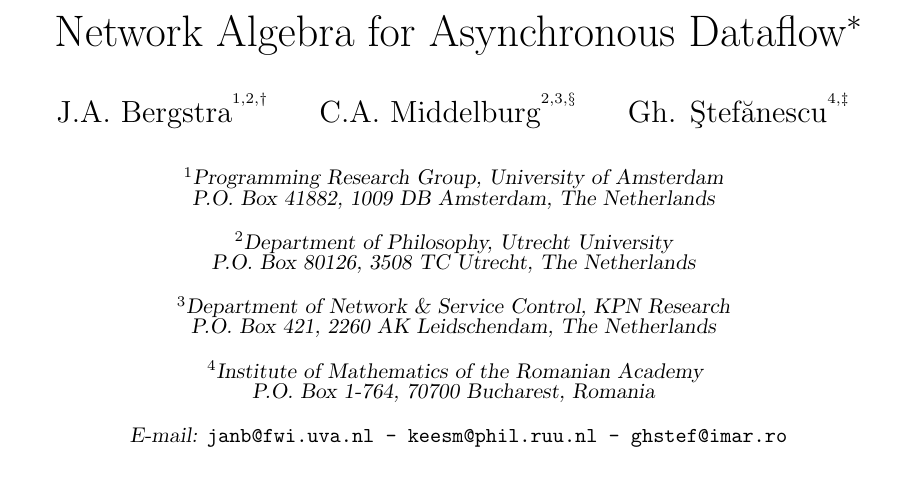
\includegraphics[width=0.6\textwidth]{Bergstra.png}}
      \end{figure}
    \end{column}
    \pause
    \begin{column}{.45\textwidth}
      \begin{itemize}
        \item Our operators can be seen as a domain specific variant of choice trees
        % \item Monadic composition
      \end{itemize}
      \vspace*{-2ex}
      \begin{figure}
        \centering
        \shadowbox{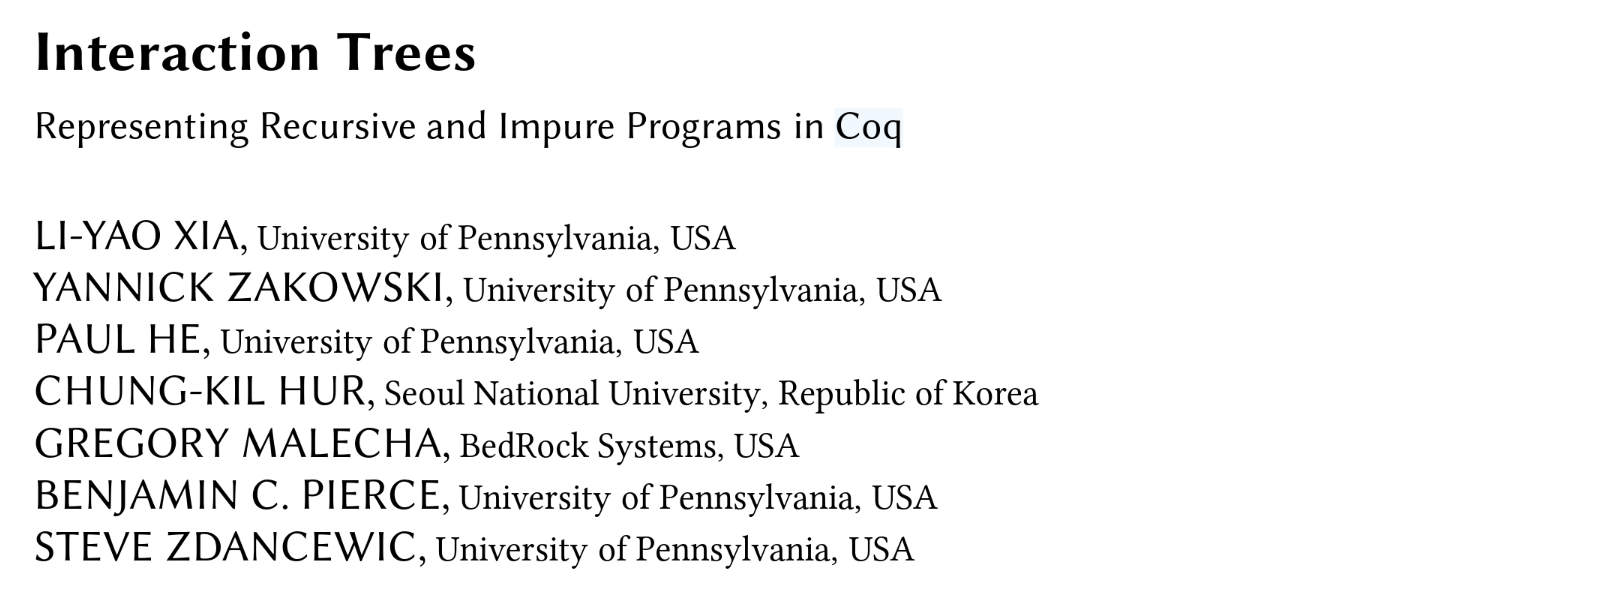
\includegraphics[width=0.6\textwidth]{itrees.png}}
      \end{figure}
      \vspace*{-3ex}
      \begin{figure}
        \centering
        \shadowbox{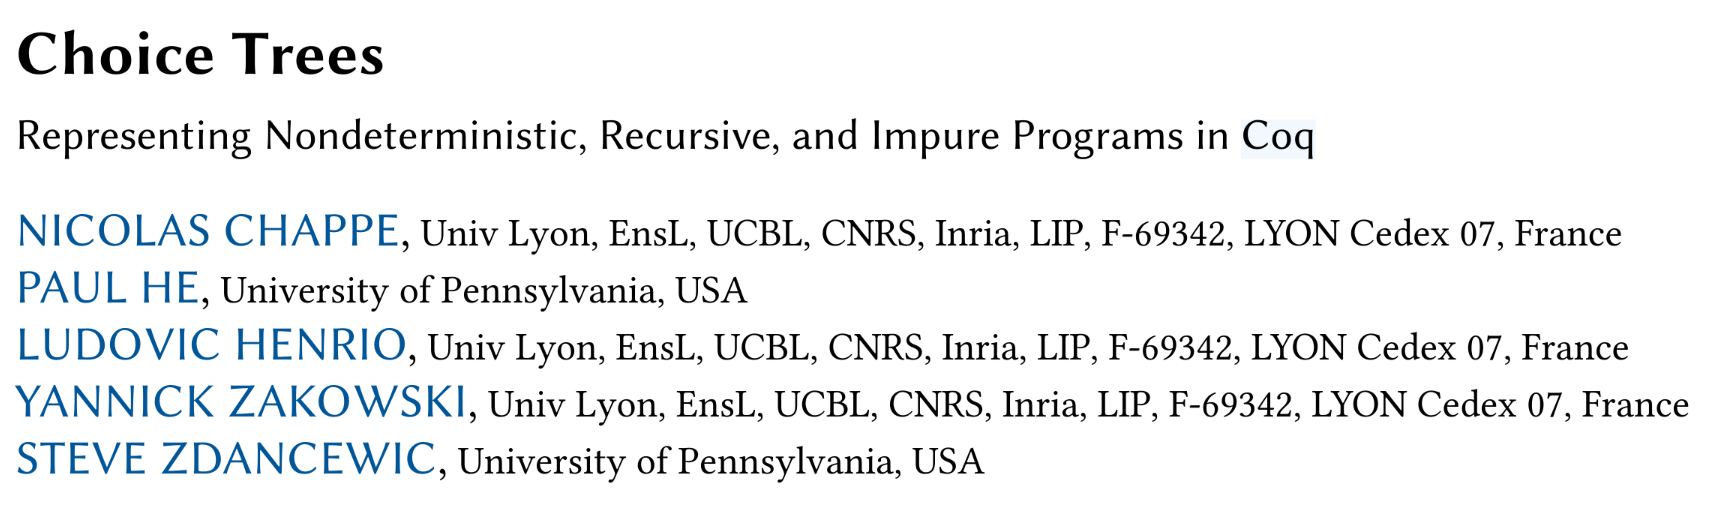
\includegraphics[width=0.6\textwidth]{ctrees.png}}
      \end{figure}
    \end{column}
  \end{columns}
    \pause
      \vspace*{-2ex}
  \begin{columns}
    \begin{column}{.45\textwidth}
      \begin{itemize}
        \item \textbf{Synchronous} dataflow languages have some proof assistant mechanization
      \end{itemize}
      \vspace*{-2ex}
      \begin{figure}
        \centering
        \shadowbox{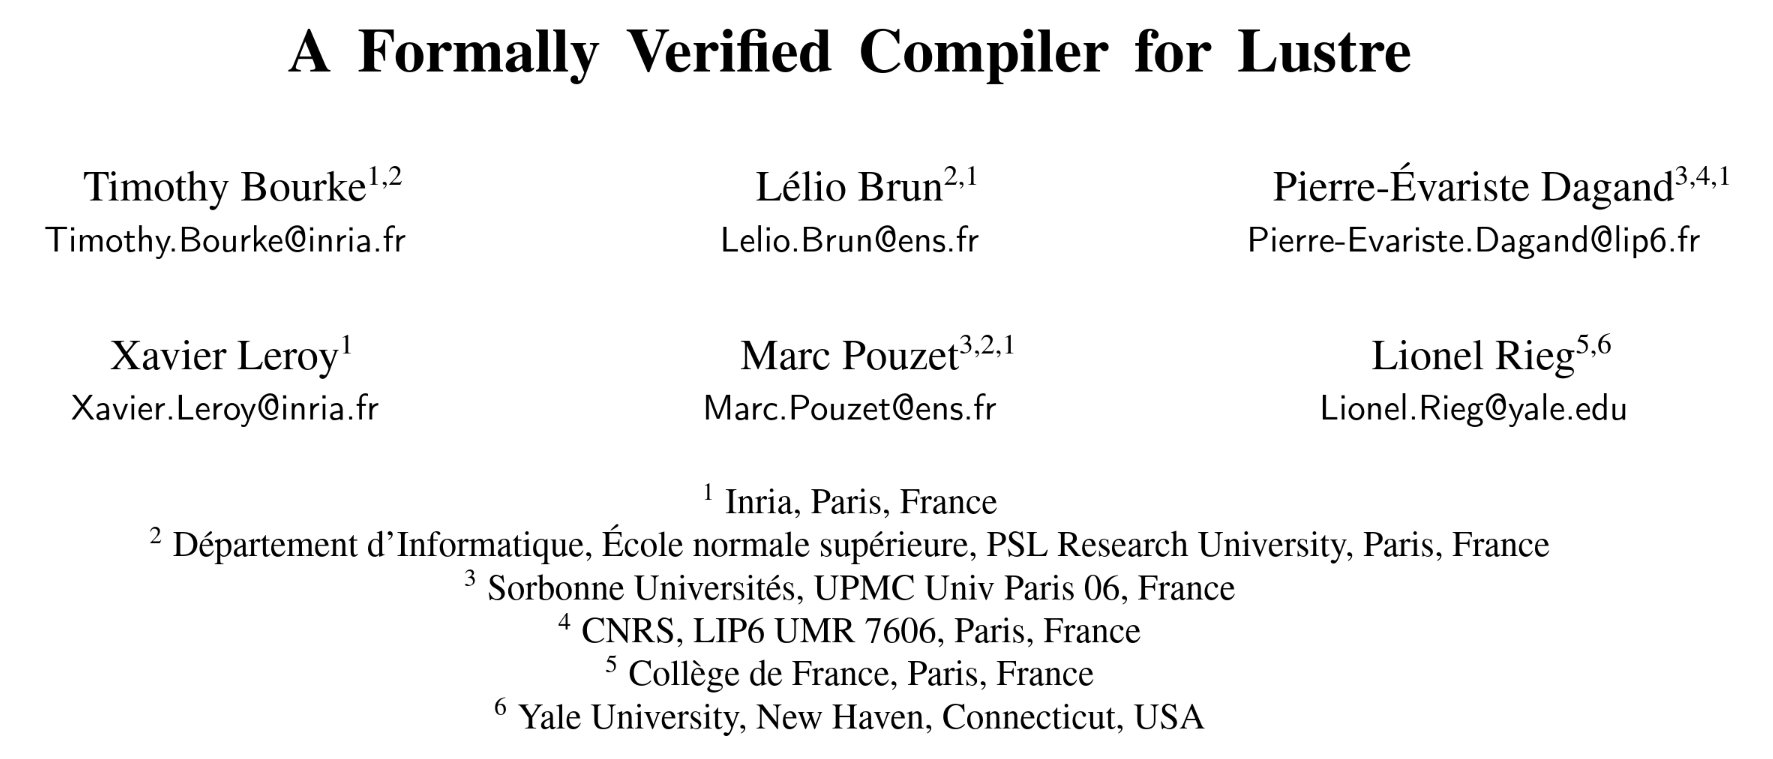
\includegraphics[width=0.5\textwidth]{velus.png}}
      \end{figure}
    \end{column}
    \pause
    \begin{column}{.45\textwidth}
      \begin{itemize}
        \item Flo: a framework for representing streaming computations originating from different systems like Flink and DBSP
      \end{itemize}
      \vspace*{-2ex}
      \begin{figure}
        \centering
        \shadowbox{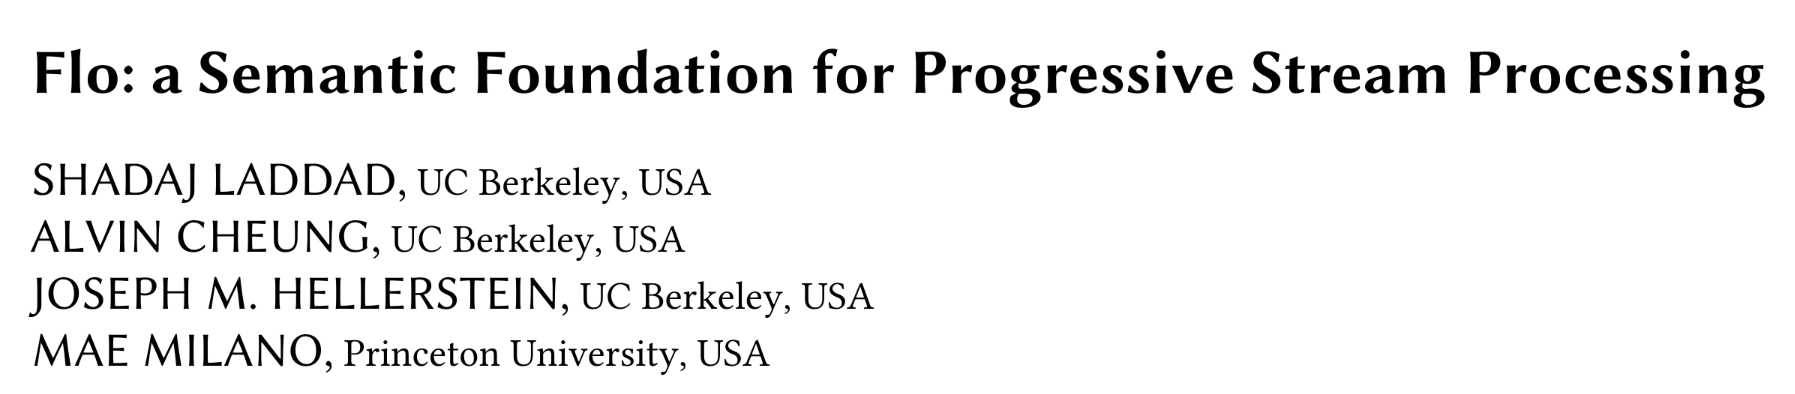
\includegraphics[width=0.5\textwidth]{flo.png}}
      \end{figure}
    \end{column}
  \end{columns}
\end{frame}

\section{Conclusion}
\begin{frame}
  \frametitle{Conclusion}
  \begin{itemize}
    \item An Isabelle/HOL instance of Nondeterministic Asynchronous Dataflow
          \pause
    \item Isabelle/HOL has a good tool set:
          \begin{itemize}
            \item Codatatypes, corecursion, coinductive predicates
          \end{itemize}
          \pause
    \item 51/52 axioms proved
          \begin{itemize}
            \item Axiom A1 for the merge operator does not hold in our instance when equivalence is $\wbisim{}{}$. \\
                  We conjecture it also does not hold in the process algebra from Bergstra et al.
          \end{itemize}
          \pause
    % \item Jonsson’s trace model, trace equivalence
          \pause
    \item Around 28 000 lines of definitions and proofs
          \pause
    \item Future work:
          \begin{itemize}
            \item Brock–Andersen Time anomaly
            \item Formalize Timely Dataflow infrastructure
            \item Verify Timely Dataflow algorithms
          \end{itemize}
  \end{itemize}
\end{frame}

\section{Questions, comments and suggestions}

\end{document}
